%% 
%% Copyright 2007-2020 Elsevier Ltd
%% 
%% This file is part of the 'Elsarticle Bundle'.
%% ---------------------------------------------
%% 
%% It may be distributed under the conditions of the LaTeX Project Public
%% License, either version 1.2 of this license or (at your option) any
%% later version.  The latest version of this license is in
%%    http://www.latex-project.org/lppl.txt
%% and version 1.2 or later is part of all distributions of LaTeX
%% version 1999/12/01 or later.
%% 
%% The list of all files belonging to the 'Elsarticle Bundle' is
%% given in the file `manifest.txt'.
%% 
%% Template article for Elsevier's document class `elsarticle'


\documentclass[preprint,12pt,authoryear]{elsarticle}

%% Use the option review to obtain double line spacing
%% \documentclass[authoryear,preprint,review,12pt]{elsarticle}

%% For including figures, graphicx.sty has been loaded in
%% elsarticle.cls. If you prefer to use the old commands
%% please give \usepackage{epsfig}

%% The amssymb package provides various useful mathematical symbols
\usepackage{amssymb}
\linespread{1.2}

%% The amsthm package provides extended theorem environments
%% \usepackage{amsthm}

%% The lineno packages adds line numbers. Start line numbering with
%% \begin{linenumbers}, end it with \end{linenumbers}. Or switch it on
%% for the whole article with 


\usepackage{lineno}
\usepackage{graphicx}
\usepackage[colorlinks=true, allcolors=blue]{hyperref}
\usepackage[a4paper, total={6.in, 9in}]{geometry}
% \linenumbers
\journal{Estuaries and Coasts}

\begin{document}

\begin{frontmatter}

%% Title, authors and addresses

%% use the tnoteref command within \title for footnotes;
%% use the tnotetext command for theassociated footnote;
%% use the fnref command within \author or \affiliation for footnotes;
%% use the fntext command for theassociated footnote;
%% use the corref command within \author for corresponding author footnotes;
%% use the cortext command for theassociated footnote;
%% use the ead command for the email address,
%% and the form \ead[url] for the home page:
%% \title{Title\tnoteref{label1}}
%% \tnotetext[label1]{}
%% \author{Name\corref{cor1}\fnref{label2}}
%% \ead{email address}
%% \ead[url]{home page}
%% \fntext[label2]{}
%% \cortext[cor1]{}
%% \affiliation{organization={},
%%            addressline={}, 
%%            city={},
%%            postcode={}, 
%%            state={},
%%            country={}}
%% \fntext[label3]{}

    \title{Seepage through the Sand Barrier at the Mouth of the Russian River, an Intermittently Closed Estuary
}

%Title suggestions: 
% Seepage through the Sand Barrier that Blocks the Mouth of the Russian River, an Intermittently Closed Estuary
% Seasonal variability of seepage across the berm in a Northern California intermittently closed estuary
% Navigating estuarine closures: Berm Seepage in a Mediterranean intermittently closed estuary.

%% use optional labels to link authors explicitly to addresses:
\author[ars]{Octavia Crompton}
\affiliation[ars]{
            organization={USDA-ARS Hydrology and Remote Sensing Laboratory},
            % addressline={},
            % city={},
            % postcode={},
            % state={},
            % country={}
            }

\author[epa]{Dane Behrens}

\affiliation[epa]{organization={Environmental Science Associates, San Francisco},
            % addressline={}, 
            % city={},
            % postcode={}, 
            % state={},
            % country={}
            }
            
\author[bml]{John Largier}
\affiliation[bml]{
            organization={Bodega Marine Laboratory, Coastal \& Marine Sciences Institute, University of California Davis},
            % addressline={},
            % city={},
            % postcode={},
            % state={},
            % country={}
            }
            
%% \affiliation[label2]{organization={},
%%             addressline={},
%%             city={},
%%             postcode={},
%%             state={},
%%             country={}}



\begin{abstract}

 
 Intermittently closed estuaries (ICEs) -- bar-built estuaries that periodically close --  are common along mountainous coastlines such as California's. While providing valuable salmonid habitat, periodic estuary closures can exacerbate challenges related to water quality and flood risk. Tools to forecast water levels during closures can support management decisions, such as whether to manually breach an estuary berm. One outstanding knowledge gap in the development of such tools is how much water seeps through the berm during closures.

Here, we use a mass-balance approach to estimate seepage through the sand barrier (berm) of the Russian River estuary, a  wave-dominated estuary in northern California that closes 1-15 times per year, with closure durations of 1-30 days. 
Using Darcy's Law  to describe flow through the berm, we estimate  an `integrated' berm hydraulic conductivity $\tilde K$ that reflects the combined influences of berm dimensions and sand conductivity. Seasonally, $\tilde K$ decreases over subsequent closures, possibly due to clogging of the sand barrier by fine sediments. This affect can persist over multiple years, although interannual variation in  $\tilde K$ likely includes variation in the shape of the berm, which can be washed away during winters with heavy rains and reform the following spring.

\end{abstract}

%%Graphical abstract
% \begin{graphicalabstract}
%\includegraphics{grabs}
% \end{graphicalabstract}

%%Research highlights
\begin{highlights}
\item Berm seepage rates are quantified for an  intermittently-closed estuary in Northern California
\item The integrated hydraulic conductivity of the berm decreases seasonally over subsequent inlet closures
\item Seepage accounts for 20-60\% of river discharge during inlet closures
\end{highlights}

\begin{keyword}
Intermittently closed estuaries \sep  Inlet closure \sep  Bar-built estuary \sep  Estuary water level
\end{keyword}

\end{frontmatter}

%% \linenumbers

% 2. Figure 2 – merge with Figure 6 photos (subsequent closures), and break of panel C into new figure
% 3. Figure annotate photos with seepage rates.  Get rid of panel A
% 5. table of top 10 closure events?
%  

\section{Introduction}
\label{sec:intro}

In many smaller estuaries in Mediterranean climates and along mountainous coasts, the mouth is intermittently closed by a wave-built sand barrier \citep{mcsweeney2017intermittently, largier2023recognizing}. 
These intermittently closed estuaries (ICEs) are common in California 
\citep{heady2015assessing}, and serve as important rearing habitats for juvenile salmonids \citep{bond2008marine, heady2015assessing, huber2020environmental}. Management options in these estuaries are often constrained by anthropogenic alterations of the physical system, including the development of adjacent low-lying flood-prone areas \citep{largier2019considerations}.



% Where they're found and conditions for closure
ICEs are typically found where estuary basins are small and the shore is exposed to high wave energy \citep{cooper2001geomorphological}. During dry-season periods of low river inflow, these small basins may lack sufficient tidal prism to maintain the mouth channel between the estuary and the ocean. Closure events occur when wave power overwhelms the combined forces of river and tidal flows through the mouth \citep{behrens2013episodic, behrens2015quantified}.  This  is especially common in regions with weaker tides (micro-tidal and meso-tidal) and stronger wave action, such as the exposed coasts of California 
\citep{mcsweeney2017intermittently}. 
Peak water levels in these estuaries often occur during closed-mouth conditions \citep{booysen2020methods}, posing significant flood risks in developed floodplain areas adjacent to the estuary \citep{clark2019systematic}. However, such conditions can also play a critical role in sustaining wetlands as sea levels rise \citep{thorne2021wetlands}. Closures thus represent a critical management challenge in ICEs, where policy and management actions can alter closure frequency and persistence, with consequences for conservation, recreation, flooding, boating, and fisheries \citep{stein2021advancing}.

% Water balance for persistent closure
Long-term closure events in estuaries require a balance between water gains --through river inflow and wave-driven overwash -- and losses through evaporation and seaward seepage through the sand barrier. 
In arid regions where river inflow is low and evaporation rates are high, evaporation can equal or exceed inflow, particularly in estuaries with larger surface areas \citep{largier2023recognizing}. 
Alternatively, seaward flow over the barrier (overflow) can balance inflow, forming a `perched estuary', which can persist when overflow velocities are too weak to erode the barrier. Here, we address the loss of water from a closed estuary via seepage, where  the head difference between estuary and ocean water levels drives water flows through the sand barrier \citep{perissinotto2010temporarily}. 
 Despite its importance in persistent closures and flood management in ICEs, seepage has received limited quantitative attention, representing a key knowledge gap. 


The Russian River is one of many intermittently closed estuaries along California's coastline \citep{johnson1973characteristics, goodwin1996predicting, heady2015assessing}. The estuary has been monitored for many years, providing an opportunity to quantify seepage rates \citep{largier20205}. River discharge is managed for water supply in summer and to mitigate flood risk in winter \citep{harassment2021russian}.  Management of the Russian River estuary requires balancing the habitat value for juvenile steelhead trout (O. mykiss) with the need to prevent high water levels that result in flooding during closure periods \citep{largier20205}. Historically, the river estuary opened and closed with the seasons.  However, due to flood risks posed to structures and farmland adjacent to the estuary, the berm is mechanically breached when estuarine water levels exceed 2.74 m above mean sea level, following an inter-agency agreement (personal communication, Sonoma County Water Agency). Thus, artificial breaching typically limits the duration of estuary closures, and is known to impact estuarine habitats and downstream ocean ecosystems  \citep{largier2023recognizing, slinger2017modes}.  Very high water levels during closures are a potentially important source of accretion to marshes in outpacing sea level rise \citep{thorne2021wetlands}.
  

Here, we quantify water loss from the Russian River during 35 persistent closure events, using 12 years of compiled data on river flow rates and estuary and ocean water levels. Using a mass balance approach, we estimate the loss rate and demonstrate that it increases with estuary water level, consistent with head-driven seepage. We then define an integrated berm hydraulic conductivity $\tilde K$ that reflects the combined influences of berm dimensions and material, and examine how $\tilde K$ varies seasonally and interannually.

\begin{figure}
    \centering
    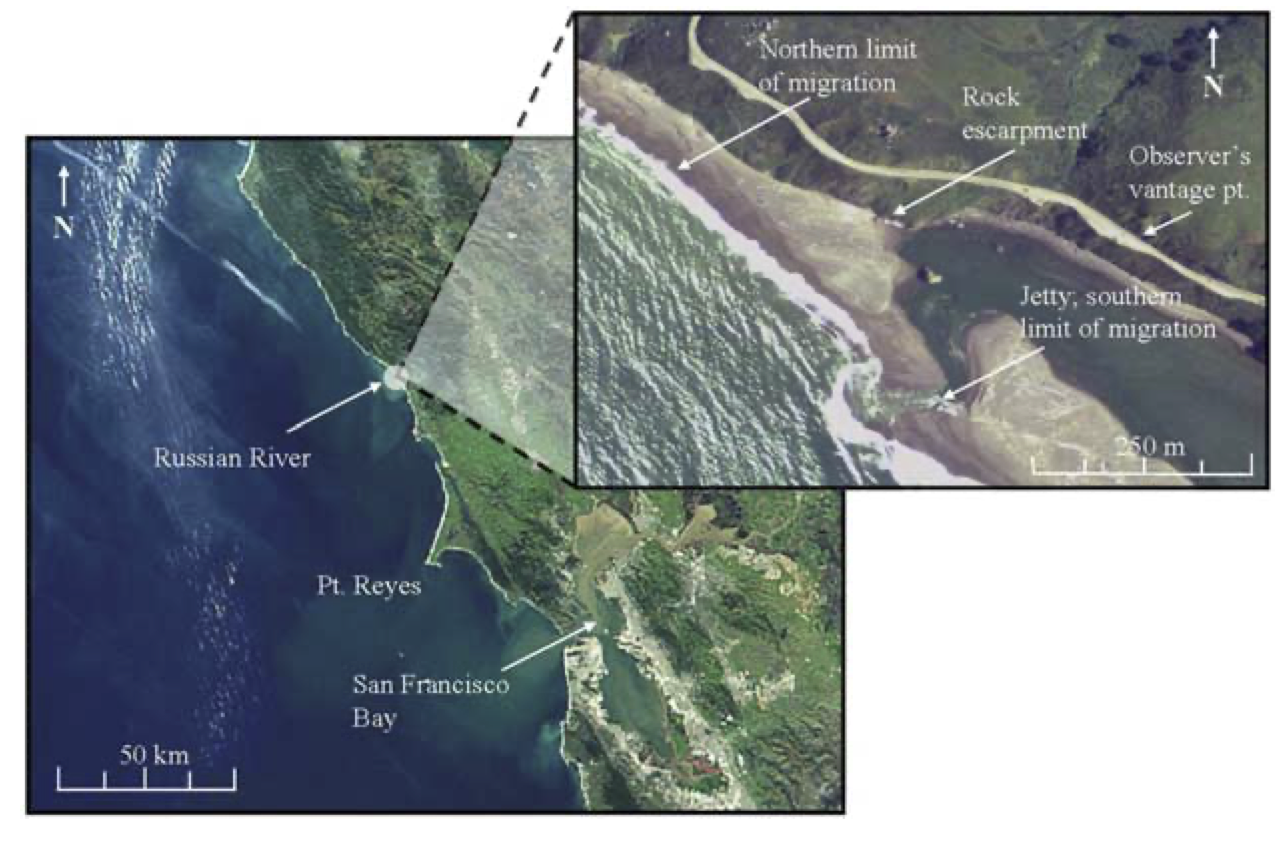
\includegraphics[width = 25pc]{figures/study_area.png}
    \caption{Location and physical characteristics of the study site. Image on the left available from NASA at \url{http:// visibleearth.nasa.gov/}. 
    Location of inlet is at approximately 38°27'00''N, 123°07'00''W. Adapted from \citet{behrens2009characterization}.
    }
    \label{fig:study_area}
\end{figure}


\section{Methods}
\label{sec:methods}

\subsection{Study Area}
\label{sec:study_area}

The Russian River extends over 175 km within a basin of 3,850 km$^2$ and flows into the Pacific Ocean, 90 km north of San Francisco, California \citep[see Figure 1,][]{behrens2009characterization}. Characterized by a Mediterranean climate, most of the precipitation falls during a handful of storms from November through April, and the area remains predominantly dry for the rest of the year. 
% The elevation varies from sea level up to 1,325 meters.

The estuary closes 1-15 times each year for periods ranging from 1 to 30 days \citep{behrens2009characterization, largier20205}.
 These closures occur when the river current is unable to erode and remove sediment deposited in the inlet channel,  due to weakening river flows, insufficient tidal prism, and/or increasing frictional losses in the channel \citep{behrens2013episodic}.  Closures are most common during periods of high wave activity, low tidal ranges, and reduced river flow, with wave action playing a dominant role. In October–November, a seasonal increase in wave heights, combined with sporadic rainfall events and artificial breaching activity, often results in a series of inlet opening and closure events. Closures are ended by river inflows that fill the estuary basin,  raising the water level until it overflows and scours a new channel at a low point in the berm.
 % before it is once again rebuilt during a large-wave event. 
 The seasonality, frequency and persistence of closure events are expected to change in response to sea-level rise, as well as changes in wave power and river flow due to climate change.

% When estuarine water levels exceed 2.74 m NGVD29 the mouth is breached mechanically to preclude high-water extremes (personal communication, Sonoma County Water Agency). The berm is altered by the remnants of a failed rock-wall jetty that likely constrains mouth dynamics \citep{behrens2009characterization}, and buildings as well as State Highway 1 have been constructed in the natural floodplain.

\subsection{Data}

 Ocean water level data were obtained from the Point Reyes tide gauge operated by the National Oceanic and Atmospheric Administration (NOAA), located 48 km south of the inlet and representative of the ocean at the Russian River mouth. Within the estuary, a water-level gauge operated by the Sonoma County Water Agency, located 1.5 km upstream of the inlet, has collected hourly data  since 1999.
Additionally, a gauge operated by the U.S. Geological Survey (USGS) has provided real-time data 3 km from the mouth since 2018 (site no. 11467270). Flow measurements are also available from USGS stations at Hacienda Bridge (site no. 11467000), 27 km upstream of the inlet, and Austin Creek (site no. 11467200), located 11 km from the ocean inlet and the only perennial tributary to the lower river. 

 % http://tidesandcurrents.noaa.gov
 %  http://waterdata.usgs.gov/nwis

% Closure data from webcam photos.
The  estuary closure record is based primarily on webcam photos of the Jenner estuary collected by Bodega Marine Laboratory (see examples in Figure \ref{fig:closures}A).  Where images are unavailable (e.g., due to fog), closures can be inferred from the absence of tidal signature in the estuary gauge data, as illustrated by the timeseries of estuary and ocean levels  in Figure \ref{fig:closures}B. 
Since 2012, there have been 107 closures, 63 with durations of 5 days or longer, and 30 with durations of 10 days or longer (see closure durations as a function of year in Figure \ref{fig:closures}C, and a histogram of closure event durations in Figure \ref{fig:closures}D).

\begin{figure}
    \centering
    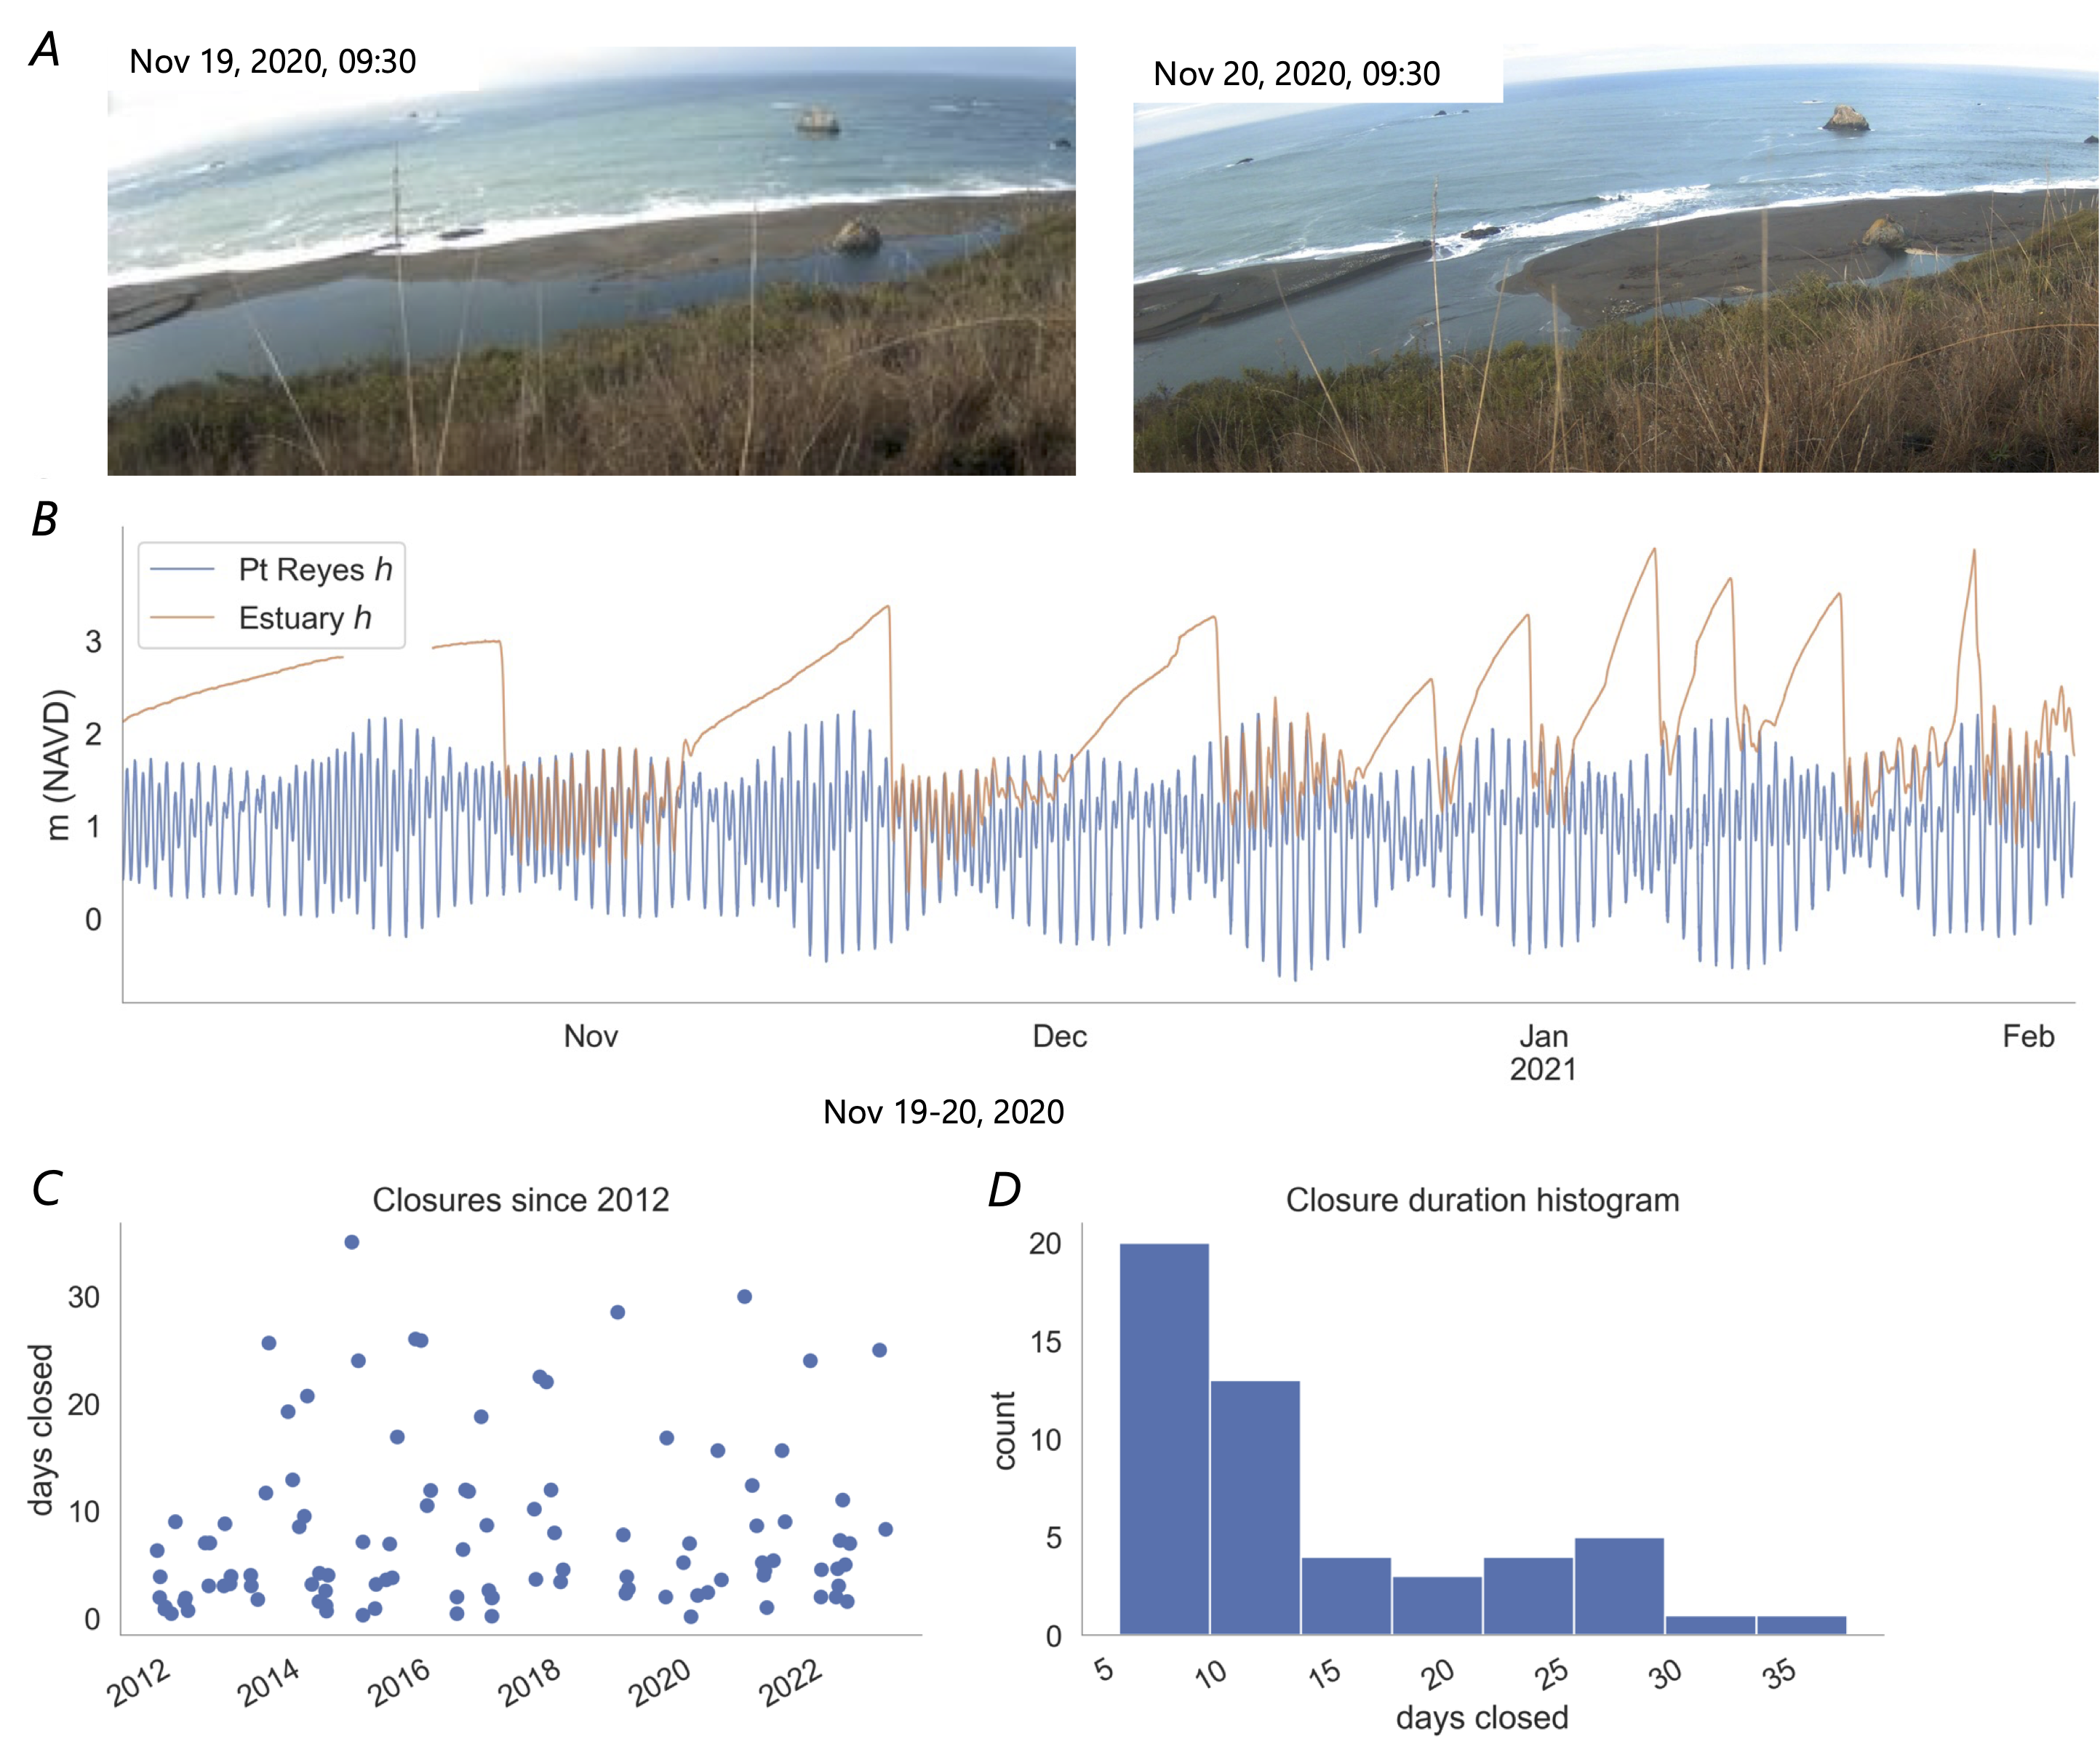
\includegraphics[width = 30pc]{figures/closure_statistics.png}
    \caption{
    (A) Illustration of closed and open states of the estuary, showing the estuary closed on November 19, 2020 (left), and open the following day (right).
    (B) Example timeseries of water level $h$ for the estuary (`Estuary $h$', orange) and ocean (`Pt Reyes $h$', blue). 
    (C) Closure duration as a function of year for estuary closures from 2012 - 2023. 
    (D) Histogram of closure durations over the same 2012 - 2023 period.
    }
    \label{fig:closures}
\end{figure}


\begin{figure}
    \centering
    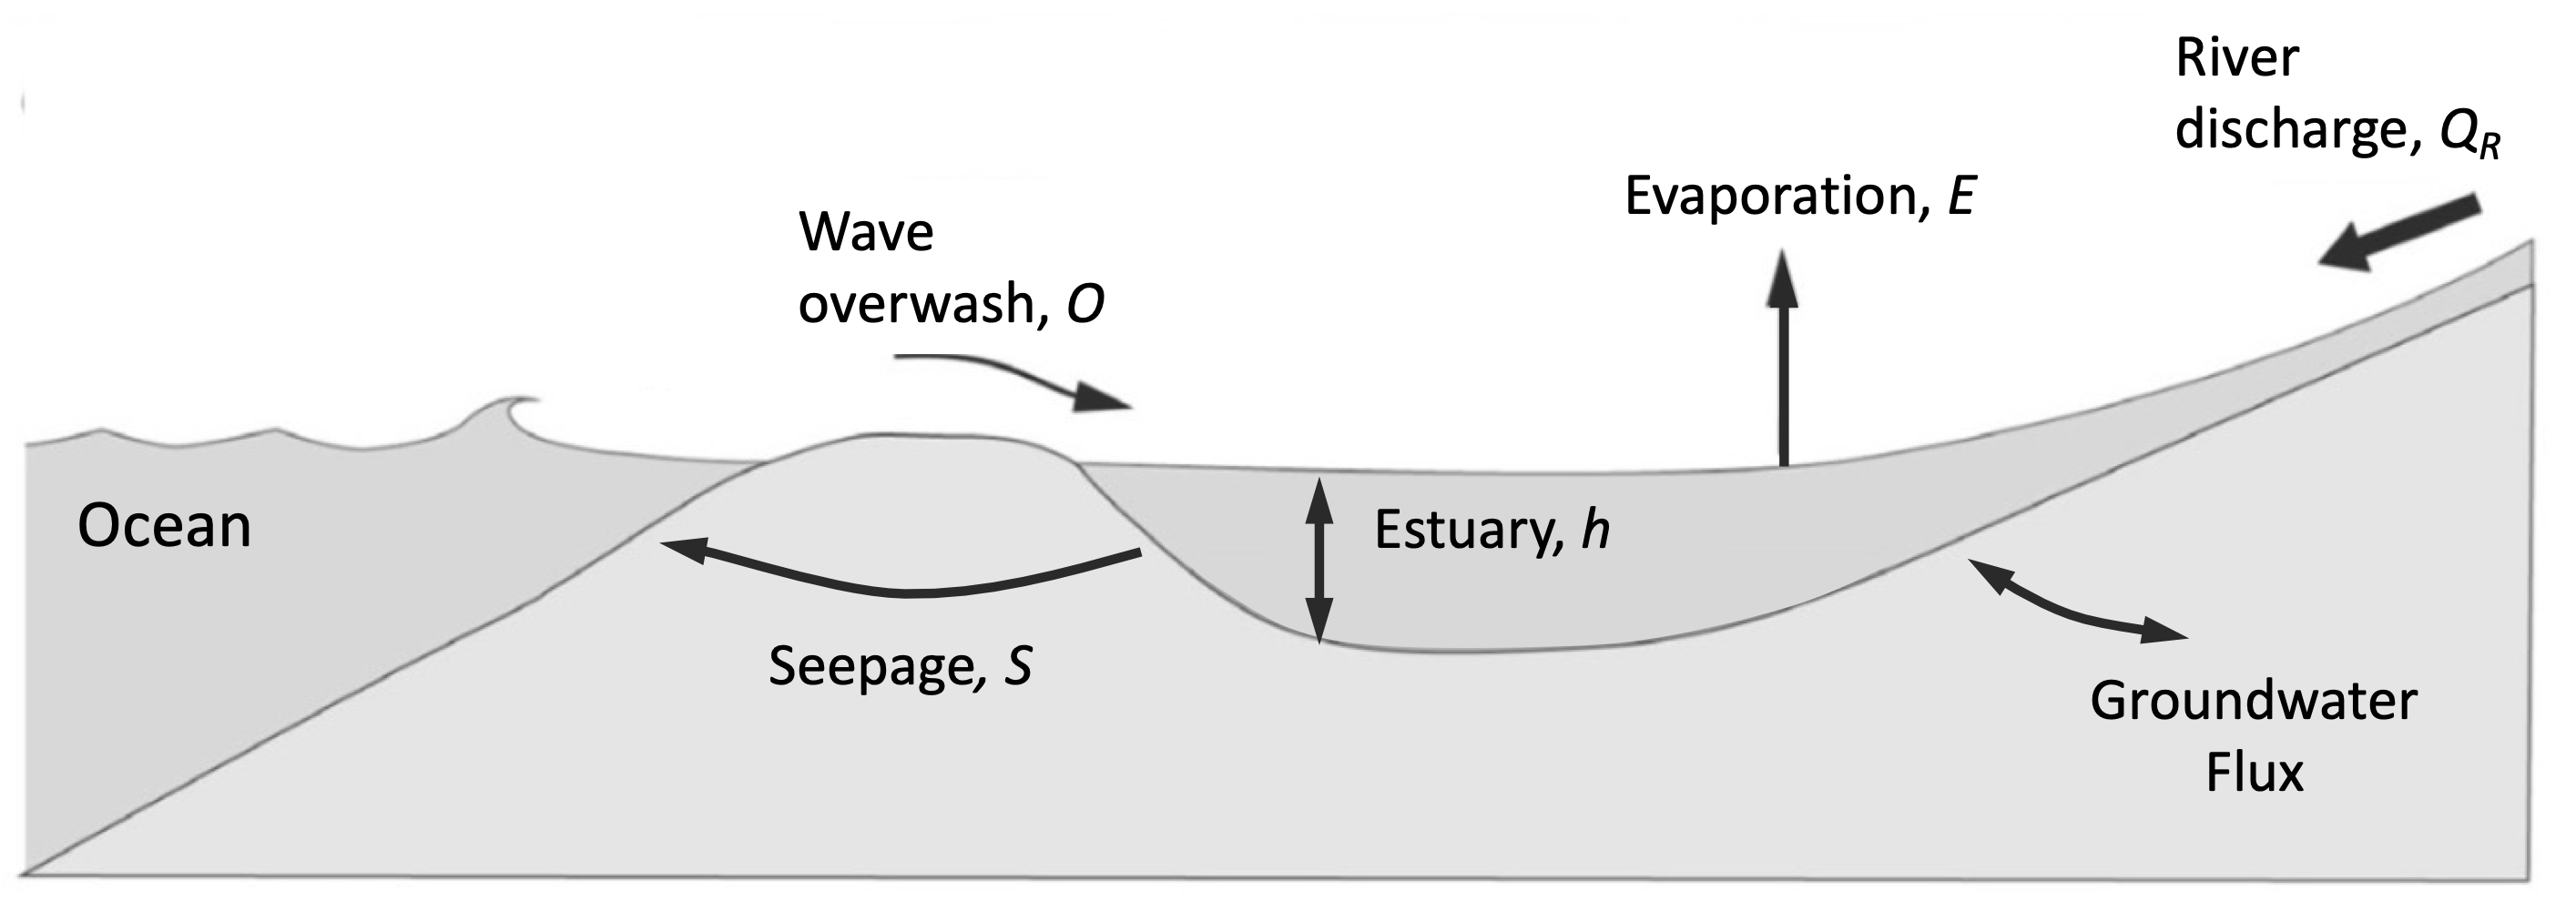
\includegraphics[width = 34pc]{figures/berm_schematic.png}
    \caption{Berm schematic illustrating terms in Equation 1.
    }
    \label{fig:schematic}
\end{figure}

\subsection{Mass balance estimation of seepage rates }

\label{sec:MB}

We estimated the seepage rate, $S$ [L$^3$/T] at daily timesteps using a mass balance approach:

\begin{equation}
\label{eq:dVdt}
    \frac{dV}{ dt} = Q_r - S + O - E A_e
\end{equation}

\noindent  where $V$  represents the estuary volume [L$^3$], 
$A_e$   the estuary surface area [L$^2$], 
$Q_r$ the river discharge [L$^3$/T],
$S$ the seepage through the berm [L$^3$/T], 
$O$ wave-driven overwash [L$^3$/T], and $E$  the evaporation rate [L/T] (see schematic in Figure \ref{fig:schematic}). Implicit in this mass balance is the assumption that groundwater-surface water exchanges are negligible and/or not persistent. 
We computed $V$ as a function of the estuary water level $h$ [L] using hypsometric data.
Figure \ref{fig:overwash}B illustrates the mass balance components for a 36-day closure from September 17 to October 22, 2014.
% A daily timestep was used as travel times through berm are expected to be of the order of a day (estimated as $W_b/K$, assuming sand $K \approx$ 45 m/day and berm width $\approx 50$ m), thus smoothing out the effect of tidal, diurnal and other high-frequency fluctuations on seepage rate. 

To identify upper limits of daily evaporation from the estuary, 
we estimated the estuary area as 100 ha and the maximum  evaporation rate as 10 mm/day, which yields $E A_e \approx 0.1$ m$^3$/s. Accordingly, we did not include evaporation in the analysis, because this term is likely an order of magnitude smaller than typical river discharge during closures ($Q_r \approx 1-5$ m$^3$/s).

Rearranging Equation \ref{eq:dVdt} yields:

\begin{equation}
\label{eq:S}
    S  = Q_r - \frac{dV}{ dt} + O.
\end{equation}

Preliminary analyses showed occasional days with  $Q_r - \frac{dV}{ dt} <0$, i.e., days in which the estuary volume increased more than river discharge can account for, which we attribute to wave overwash. Overwash can occur on days with big waves at high tide and is most common near the beginning of closures events (i.e., within the first couple of days, before wave action builds up the sand barrier crest elevation).

To exclude days with overwash, we applied a filtering approach that used river discharge $Q_r$ to forecast estuary depth on the following day. 
Specifically, river discharge and  estuary volume  on day $t$ were used to predict the estuary volume on the following day,  as $\hat V_{t+1} = V_{t} + Q_{r,t} \Delta t$.    $\hat h_{t+1}$  was then calculated from $\hat V_{t+1}$ using hypsometry data.
If seepage, evaporation, and overwash are all negligible, we expect that $h_{t+1} = \hat h_{t+1}$. If overwash is negligible and seepage is significant, then $ h_{t+1} < \hat h_{t+1} $. Conversely, if  the overwash  exceeds seepage, then $h_{t+1} > \hat h_{t+1} $.  To exclude overwash days, we removed days with $h_{t+1} > \hat h_{t+1}$ and $Q_r - \frac{dV}{ dt} < 0$ from the analysis (e.g., Figure 4C: September 18-19 and 25-26, and October 12-13).
% Excluding days with  $ h_{t+1} > \hat h_{t+1}$ is a more restrictive criteria than the simpler approach of excluding days with $Q_r - \frac{dV}{ dt} < 0$.
Visual inspection of estuary photographs confirmed overwash on all excluded days. 

 With these days filtered out, we assumed that overwash was negligible on the remaining days ($O \sim 0$); however, there may be weaker overwash on other days that reduces the estimate of seepage $S$ (e.g., Figure 4C: 20 September). Under the assumption of negligible overwash, Equation \ref{eq:S} simplifies to:

\begin{equation}
    S  = Q_r - \frac{dV}{ dt}.
\end{equation}


% This approach -- along with the unfiltered data -- are compared in supporting information Figure S4.

  \begin{figure}
    \centering
    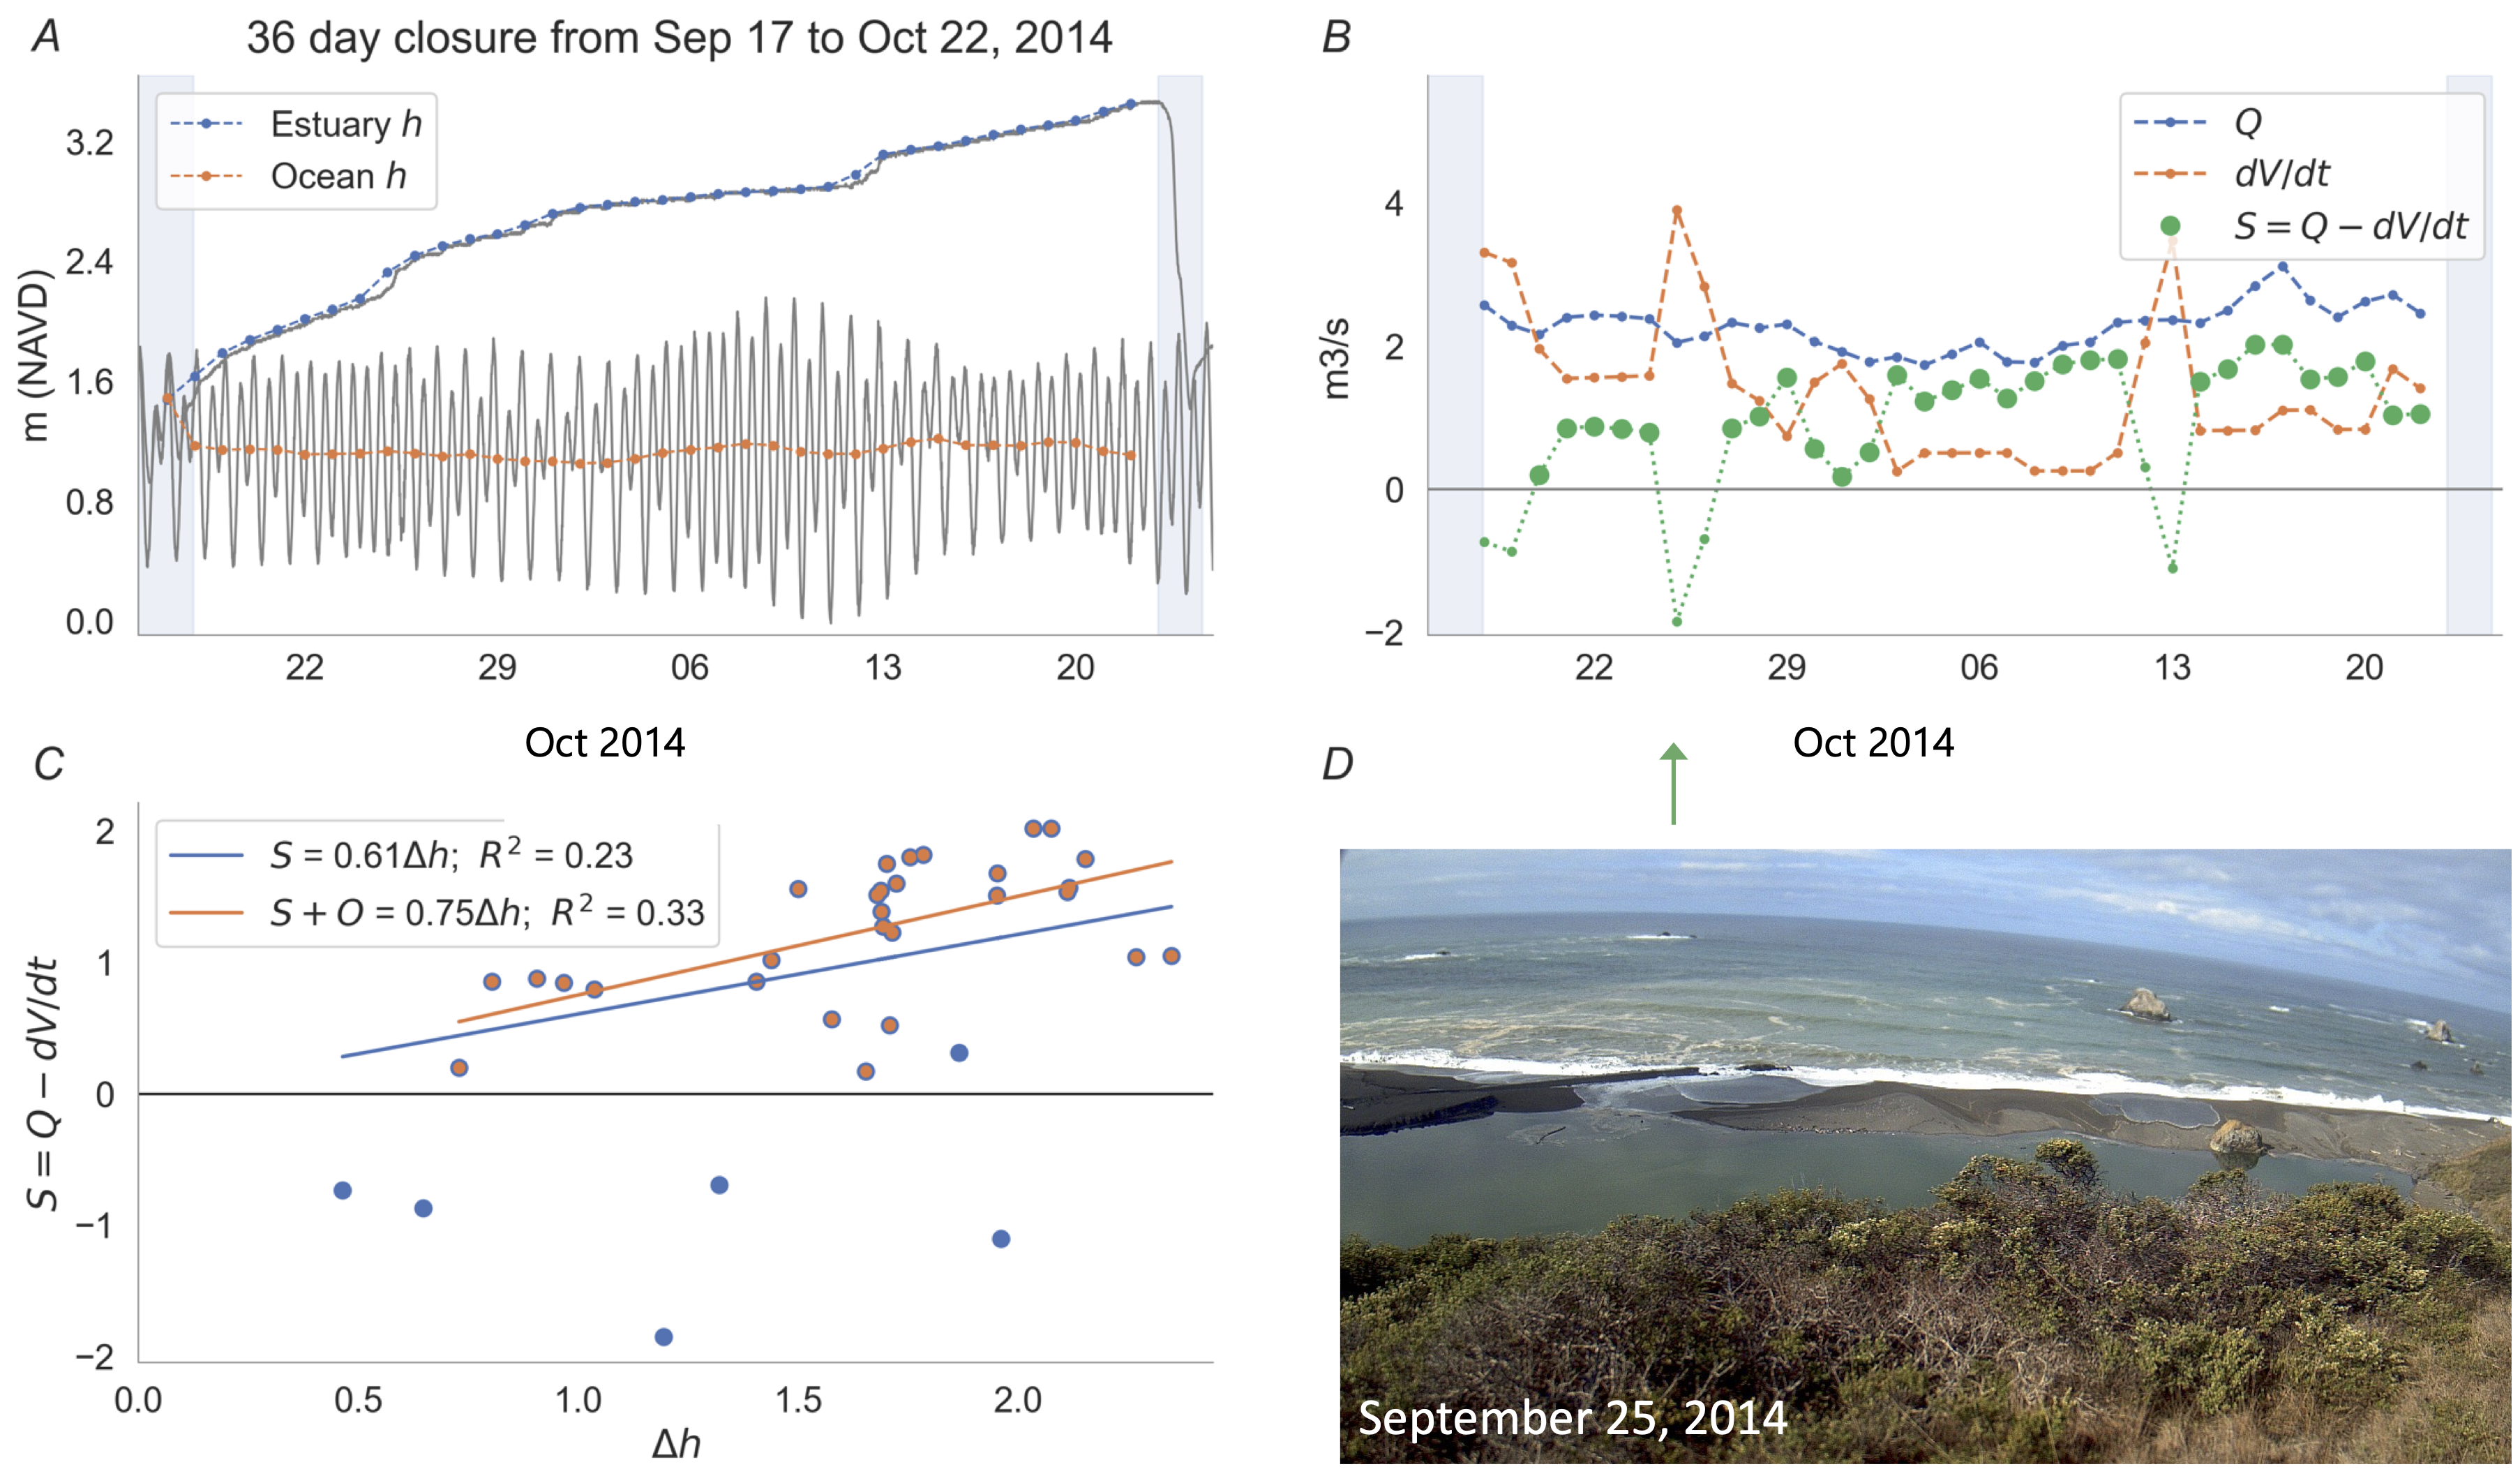
\includegraphics[width = \textwidth]{figures/overwash.png}
    \caption{(A) Timeseries of estuary depth and ocean level  during a closure from September 17 to  October 22, 2014. 
    Solid lines show 15 minute data, and dotted lines show the daily averaged data.
    Grey shading indicates periods when the estuary mouth was open.
    (B)  The mass balance components at daily intervals: the estuary volume change per day, $dV/dt$  (orange),  river discharge, $Q_r$  (blue) and seepage, $S = Q - dV/dt$ (green). In the $S$ timeseries, smaller marker sizes indicate points that were filtered out to exclude days dominated by overwash. (C) The berm integrated hydraulic conductivity $\tilde K$ was computed by fitting a regression of $S$ on $\Delta h$ for days when with $Q_r - \frac{dV}{dt} < 0$ and $h_{t+1} > \hat{h}_{t+1}$ (see Section \ref{sec:MB}).
    (D) A photo of the estuary mouth taken September 25, 2014, in which overwash is visible. 
    }
    \label{fig:overwash}
\end{figure}

\subsection{Integrated berm hydraulic conductivity }

We assume that Darcy's law applies to seepage across the berm:

\begin{equation}
    S = K A_b \frac{\Delta h}{ W_b}
    \label{eq:Darcy}
\end{equation}

\noindent where $K$ [L/T] is the mean hydraulic conductivity of the berm, $\Delta h $  [L] is the head difference between estuary and ocean, $A_b$ [L$^2$] is the cross-sectional berm area, and $W_b$ [L] is the berm width between estuary and ocean (the distance over which hydraulic pressure drops from estuary to ocean). More precisely, $A_b = L_b h_b$ is the hydraulically active cross-sectional area of flow,  where $L_b$ and $h_b$ are the length and vertical height, respectively, of water flow through the berm.

As the estuary water level rises, the hydraulic gradient increases, and one may also expect $A_b$ or $W_b$ to vary, yielding a nonlinear dependence of $S$ on estuary water level and thus on $\Delta h$. To make any such dependencies explicit, $A_b$ and $W_b$ are expressed as $A_b = A'_b \Delta h^x$ and $W_b = W'_b \Delta h^y$, where $A'_b$ and $W'_b$ are constants and the exponents $x$ and $y$ account for any potential dependencies of $A_b$ and $W_b$ on $\Delta h$. 
Equation \ref{eq:Darcy} is rewritten:

\begin{equation}
    S = K (A'_b \Delta h^x) \frac{\Delta h}{ (W'_b \Delta h^y)}.
    \label{eq:Darcy_w_exponents}
\end{equation}

However, the flow cross-sectional area and berm width are unknown, as are their dependencies on $\Delta h$.  While the berm shape can be estimated from aerial or satellite imagery, this likely differs from its hydraulically-active area. We therefore estimate an `integrated’ hydraulic conductivity $\tilde K$:

\begin{equation}
    S = \tilde K  \Delta h^b,
    \label{eq:tildeK}
\end{equation}

 \noindent where $\tilde K =  \frac{K A'_b}{ W'_b}$, and the exponent $b$ accounts for any dependencies of $A_b$ and $W_b$ on $\Delta h$ (i.e., the exponents $x$ and $y$, $b = 1 + x - y$). Note that, because the units of $\tilde K$  depend on the exponent, $\tilde K$  is not comparable between different values of $b$. 

To estimate $\tilde K$ for each closure event,
 we plotted $S$ (inferred through mass balance at daily time intervals) against $\Delta h^b$, and fit a regression line to obtain $\tilde K$ (see Figure \ref{fig:overwash}C for illustration). We adjusted the exponent $b$ from 0.5 to 2, and defined the  best-fit exponent, $b_{optim}$, as the exponent value that maximizes the model coefficient of determination, $R^2$. In the linear case with $b = 1$, $\tilde K$ is independent of  $\Delta h$ and can be interpreted as an integrated hydraulic conductivity with dimensions L$^2$/T. 
 %If the data are not filtered to exclude days with wave-driven overwash, $\tilde K$ represents an integrated hydraulic conductivity representing both seepage and overwash, $S + O$.  

\section{Results}

The best-fit exponent $b$ differs between closures (see Table \ref{tab:closures}, which lists $\tilde K$ and $R^2$ for the linear case, as well as $b_{optim}$ and $R^2_{optim}$ for the best-fit case, for all closures with at least 5 days of data). The average of the best-fit values is $b = 1.25$; however, the difference in prediction errors is minor, with the ensemble mean $R^2=0.43$ for $b = 1$ and  $R^2=0.45$ for $b = 1.25$. This is illustrated by Figure \ref{fig:compare_fits}, which compares different values of the exponent $b$ for the three longest closures (panels A-C) and all of the closure events combined (panel D). Given the comparable errors for $b = 1$ and 1.25, we adopt a linear fit, which  has the advantage that $\tilde K$ is interpretable as a hydraulic conductivity with dimensions L$^2$/T.

  \begin{figure}
    \centering
    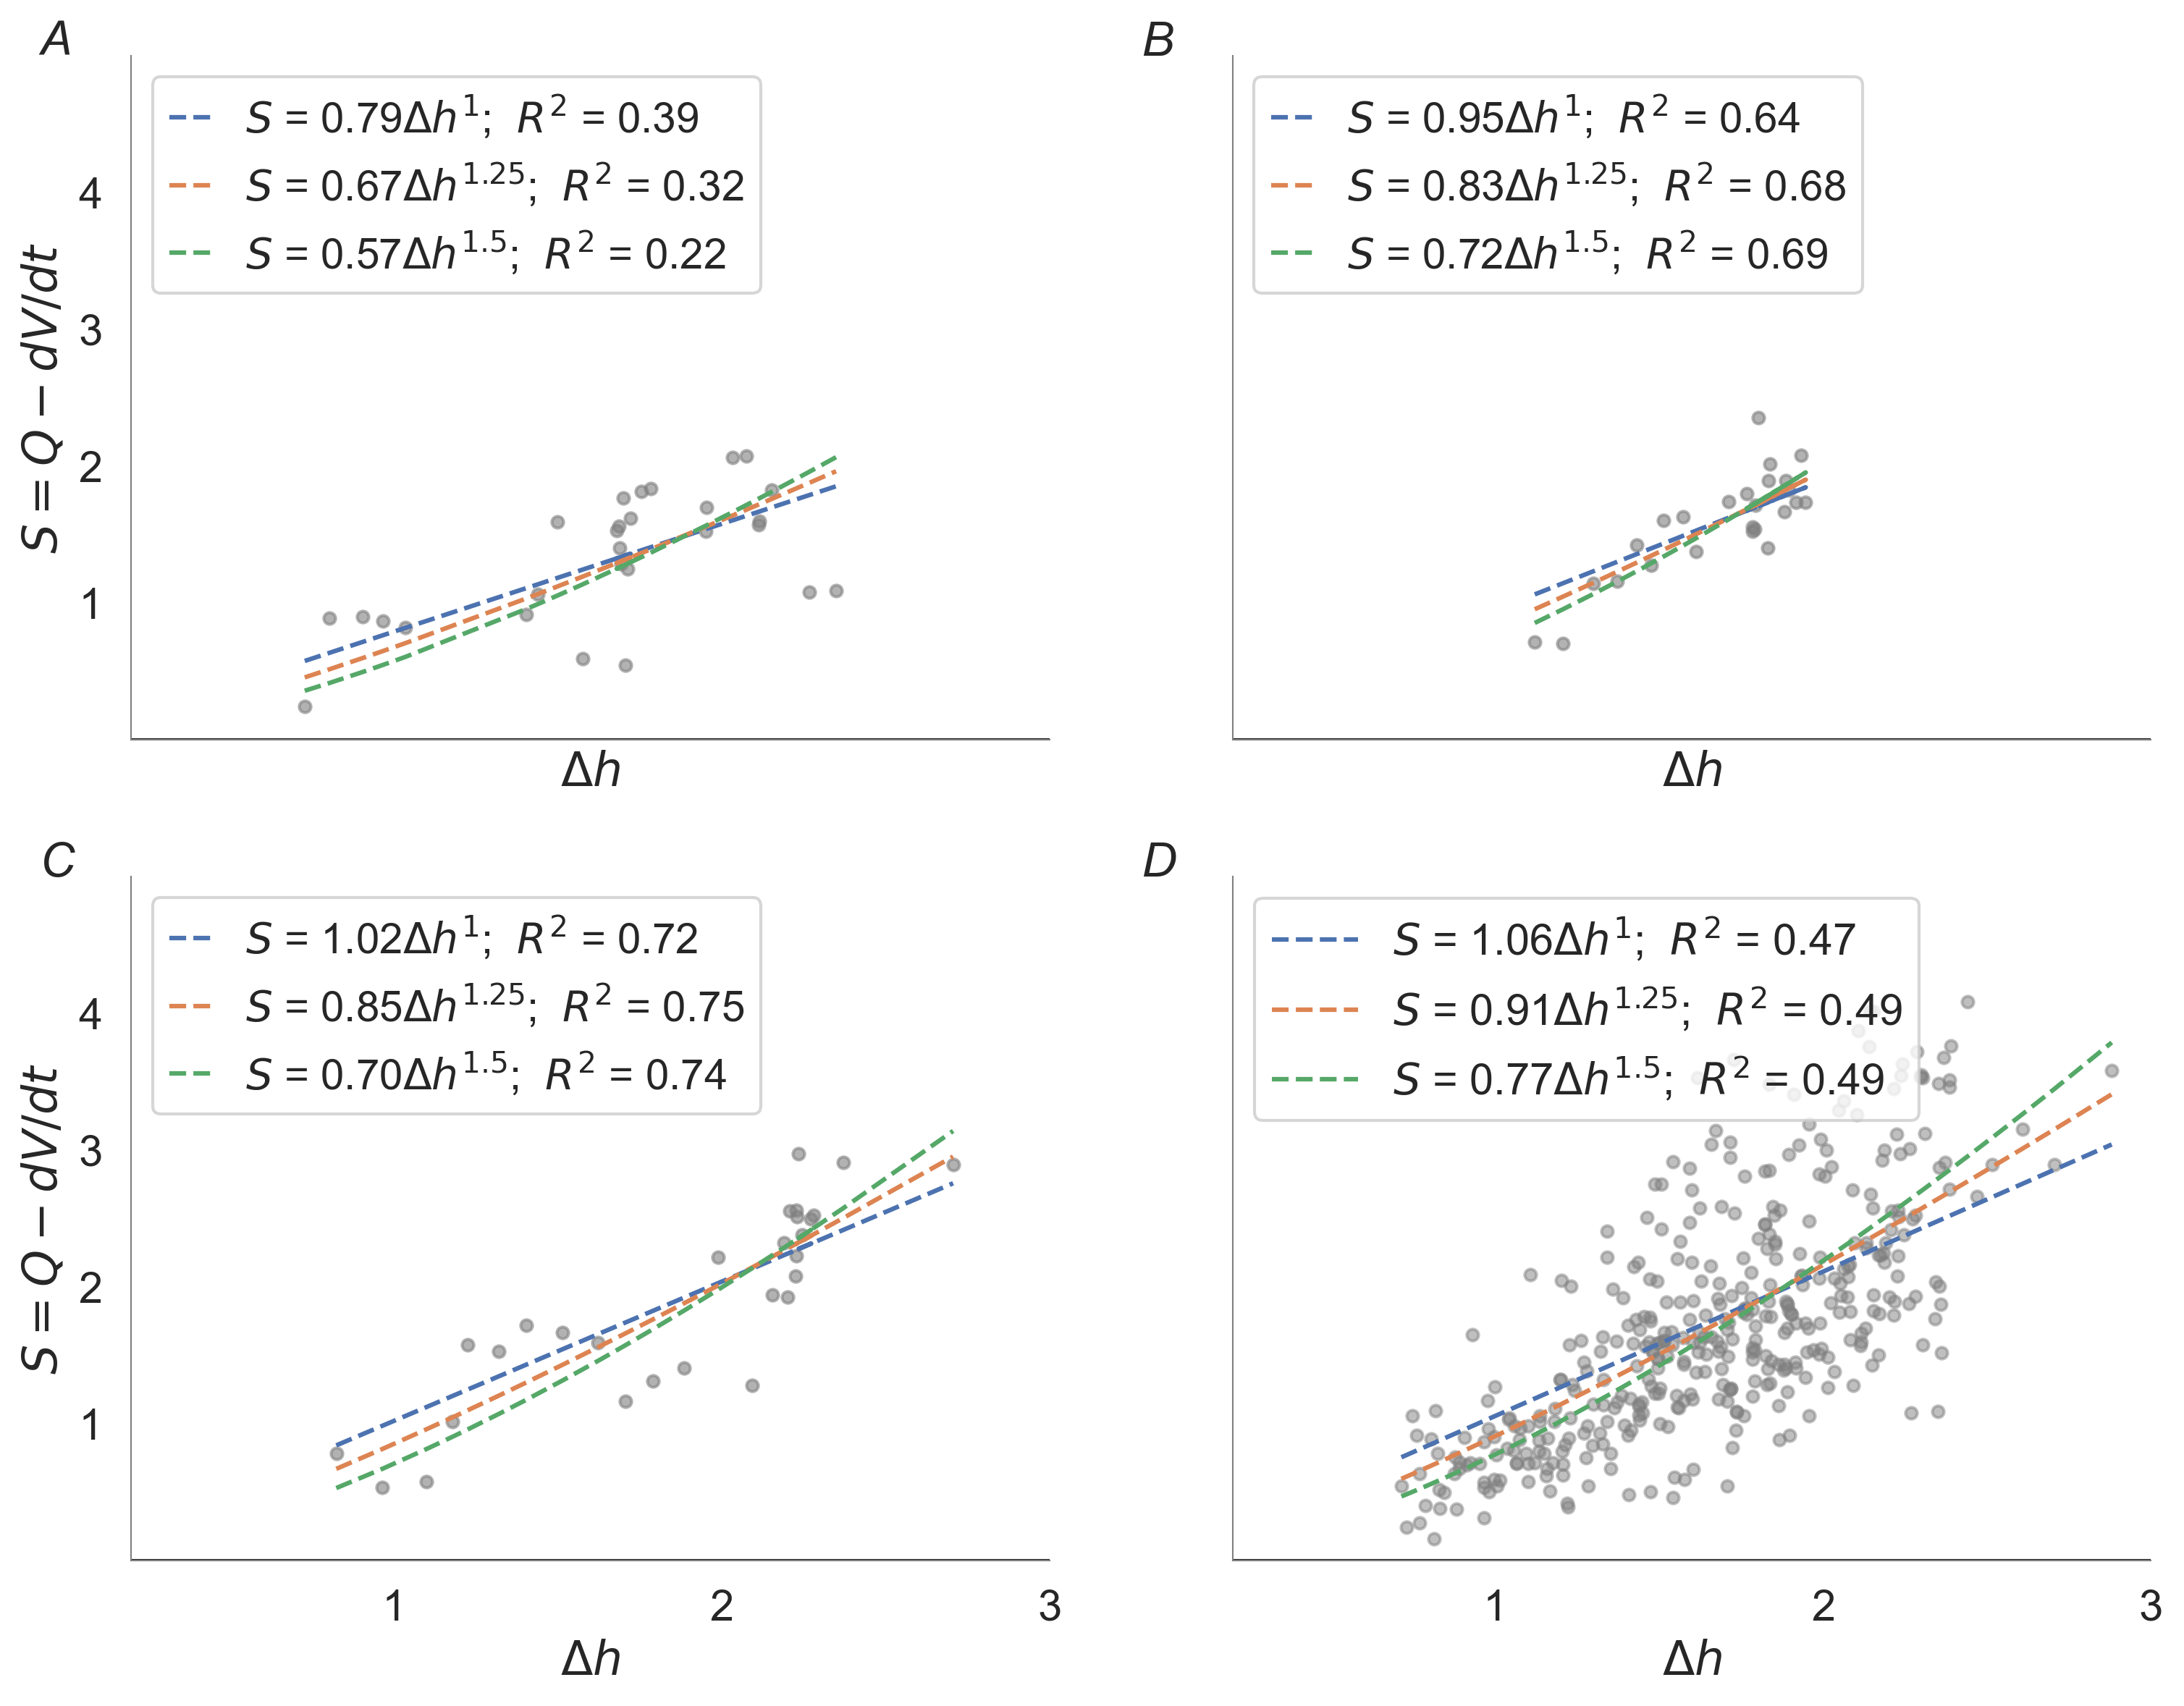
\includegraphics[width = \textwidth]{figures/compare_fits4.png}
    \caption{Comparing exponent fits for three longest closures in 2012: (A) a 36 day closure starting on September 17, 2014  (see also Figure \ref{fig:overwash}), (B) a 31 day closure starting on September 26, 2020, (C) a 29 day closure starting on October 16, 2018, and (D) all closure events combined. The closures in panels B and C are shown in further detail in SI Figures S1 and S2 (analogous to Figure \ref{fig:overwash}).
    }
    \label{fig:compare_fits}
\end{figure}

\begin{figure}
    \centering
    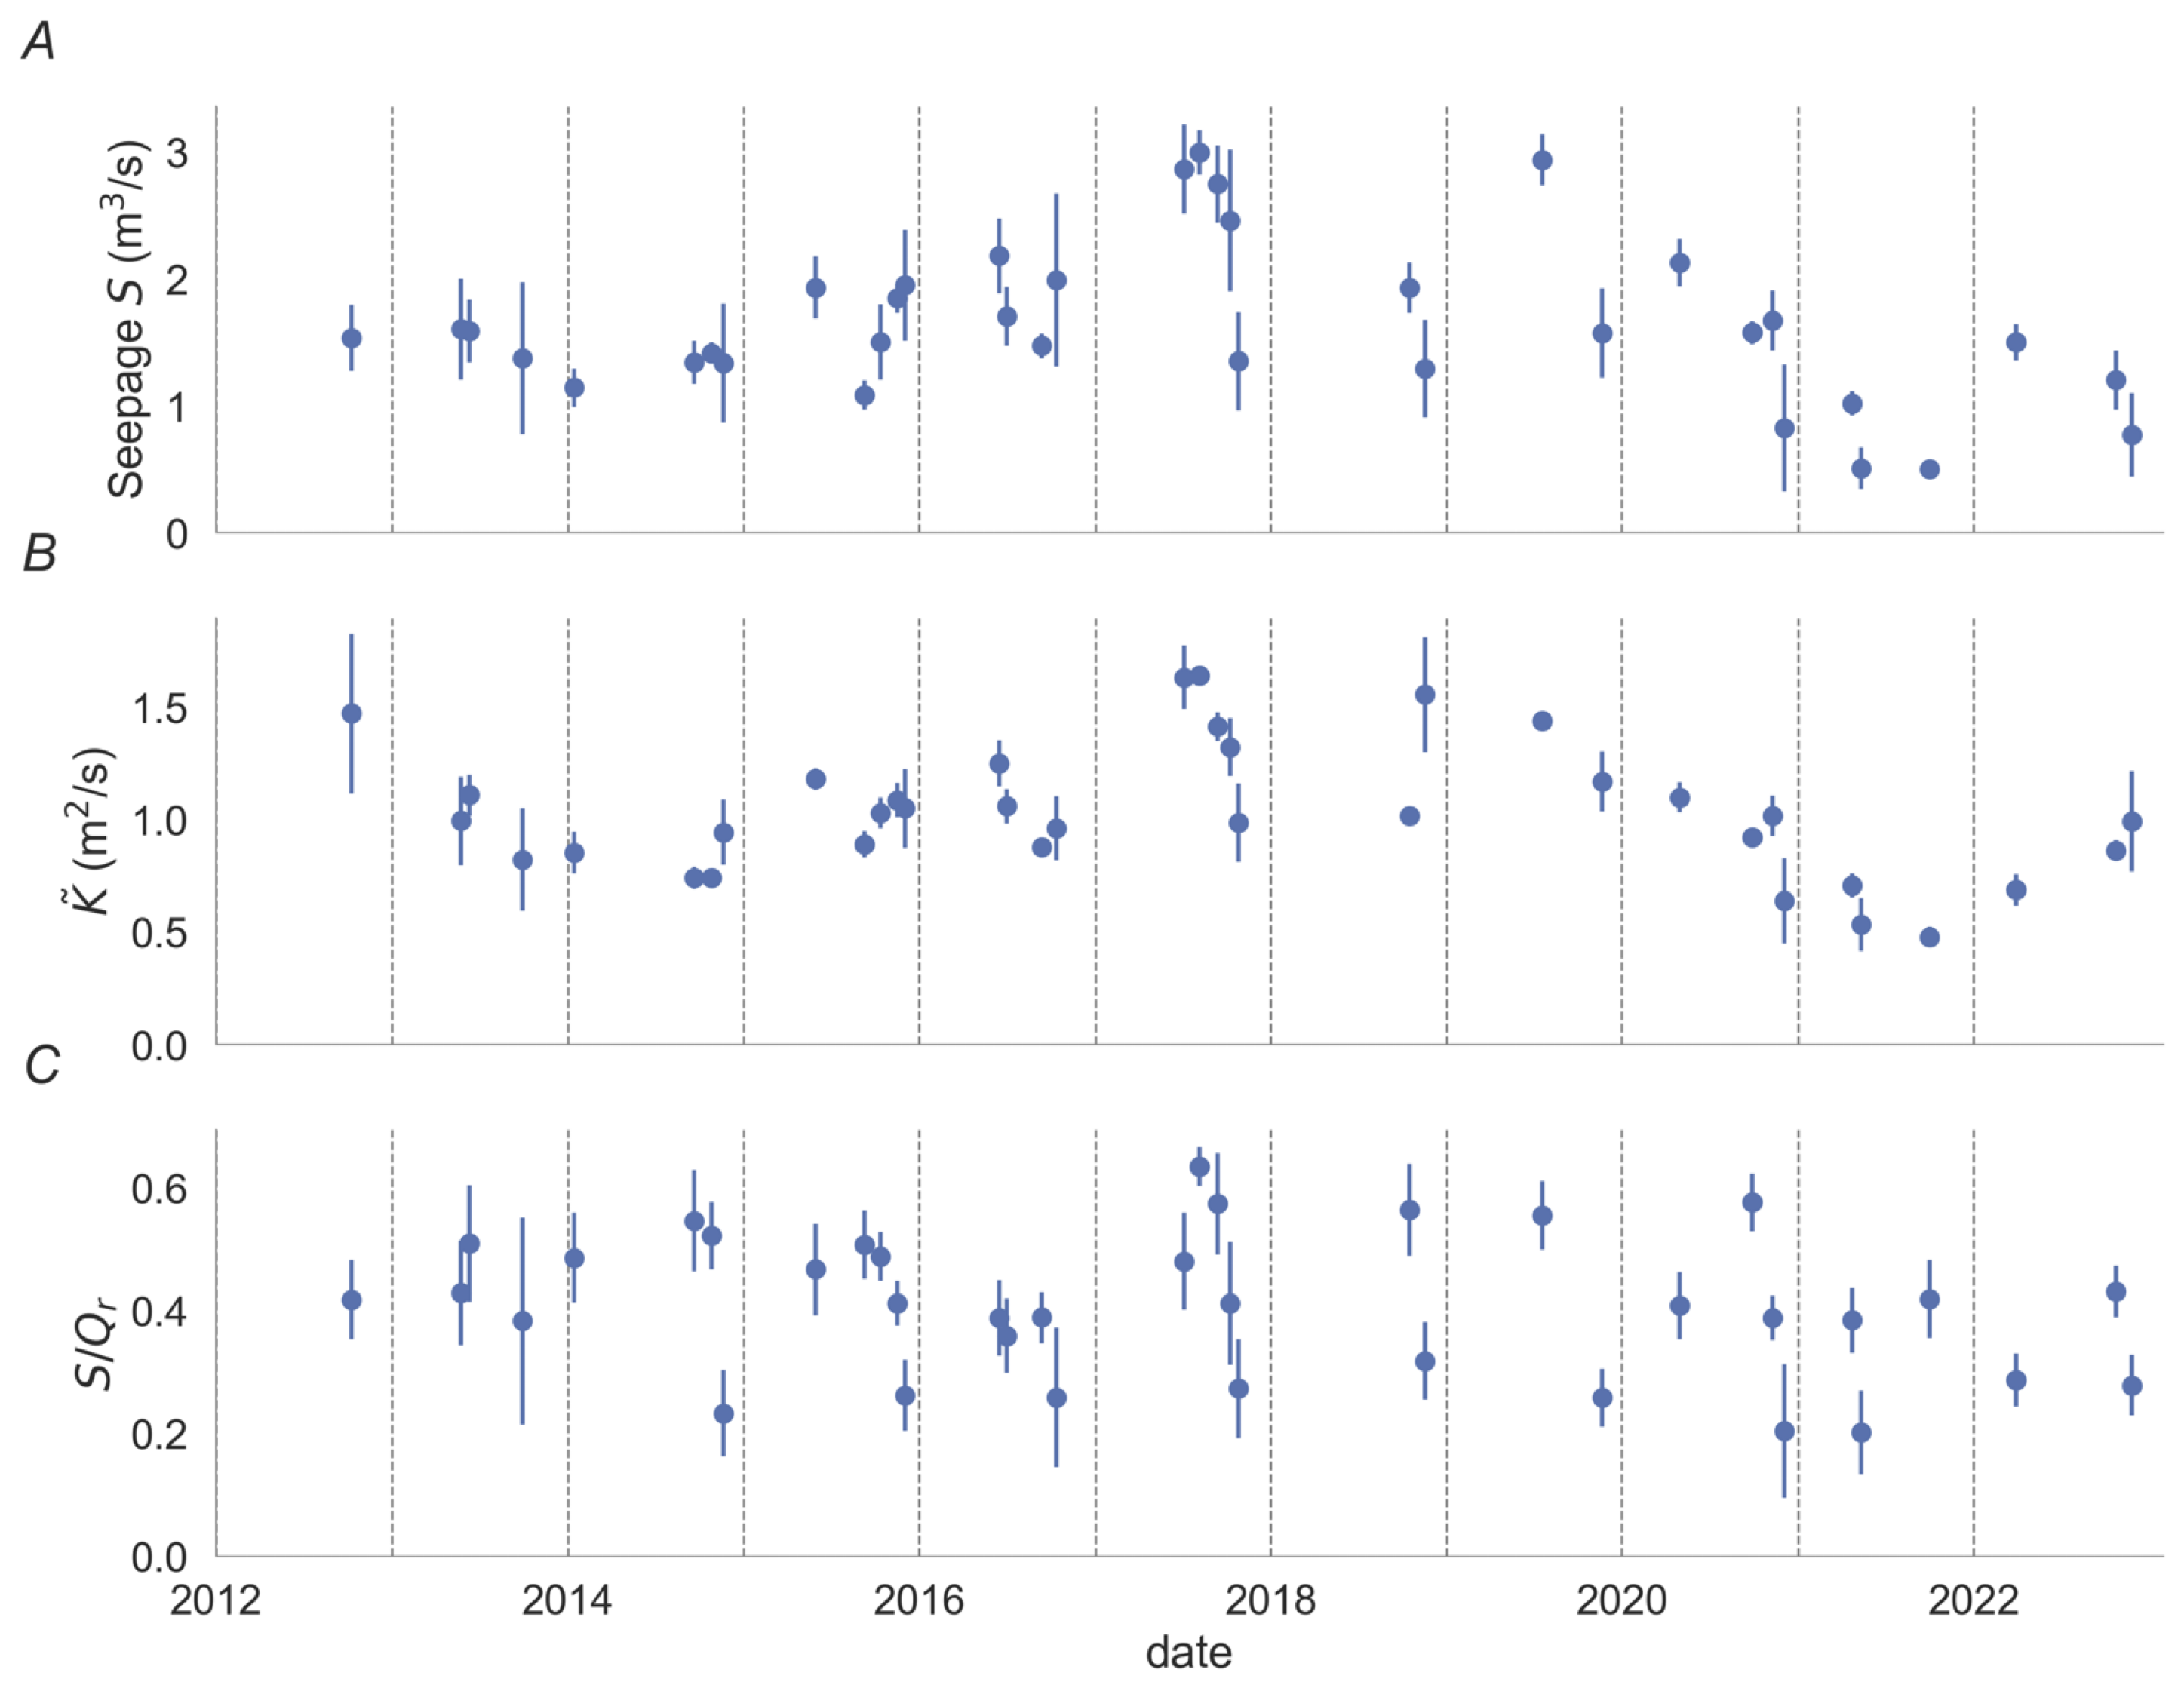
\includegraphics[width = \textwidth]{figures/summary.png}
    \caption{(A) Mean seepage rate $S$  computed for each closure, with error bars indicating bootstrapped confidence intervals on the mean.
    (B) Integrated hydraulic conductivity determined through regression of $S$ on $\Delta h$ for each closure event.  
    (C) Ratio of seepage to river discharge, $S/Q_r$. 
    Only closure events with at least 5 days of data are included.  
    }
    \label{fig:summary}
\end{figure}


Figure \ref{fig:summary} shows how the mean seepage rate $S$  (panel A) and the integrated hydraulic conductivity $\tilde K$ (panel B) vary over time for all closures with  at least 5 days of data. Seepage rates vary from 0.5 to 3.0 m$^3$/s, with the highest rates in 2017. $\tilde K$ remains relatively consistent across closures, ranging from 0.5 to 1.5 m$^2$/s. The highest conductivity was observed in 2017, consistent with the  high seepage rates that year. In some years, $\tilde K$ decreases over subsequent closures (notably, in 2016 and 2017), reflecting a seasonal change in $K$, $A_b$, and/or $W_b$. 
Figure \ref{fig:summary}C shows the ratio of seepage to river discharge, $S/Q$, which ranges from 0.2 to 0.6, with significant variability both within and between years (and again exhibiting a maximum in 2017).


Supporting information Figure S3 compares the results obtained with and without overwash days included in the analysis (i.e., $S$ versus $S + O$). $\tilde K$ values are smaller with overwash included, because $O+S < S$, and not representative of actual seepage flows.
%In the unfiltered case, seepage values are smaller because overwash is counted as `negative' seepage.  
Nevertheless, the results are qualitatively similar, showing the same seasonal and interannual trends in $\tilde K$.
 % Orange markers show the data filtered to exclude overwash ($S$), and blue shows the unfiltered results ($S + O$).  

\begin{table}[]    
    \centering
\caption{Summary statistics for the 30 longest closures, including closure start date, duration and number of data points $N$. $\tilde K$ and $R^2$ columns indicate integrated hydraulic conductivity and $R^2$ value determined fitting Equation 6 with $b = 1$.  $b_{optim}$ is exponent that achieves maximum $R^2$ value, $R^2_{optim}$. }   
    \small
\begin{tabular}{lllll|ll}
\hline
Date & Duration & $N$ & $\tilde K$ & $R^2$ & $b_{optim}$ & $R^2_{optim}$ \\
\hline
2014-09-17 & 36 & 28 & 0.79 [0.70-0.87] & 0.39 & 0.80 & 0.40 \\
2020-09-26 & 31 & 25 & 0.95 [0.89-1.00] & 0.64 & 1.40 & 0.69 \\
2018-10-16 & 29 & 28 & 1.02 [0.94-1.09] & 0.72 & 1.30 & 0.75 \\
2015-09-08 & 26 & 23 & 0.90 [0.78-1.01] & 0.05 & 0.50 & 0.21 \\
2015-10-10 & 27 & 21 & 1.09 [0.99-1.19] & 0.78 & 1.40 & 0.83 \\
2013-06-08 & 26 & 18 & 1.21 [1.00-1.42] & 0.41 & 1.40 & 0.44 \\
2022-10-21 & 25 & 18 & 0.90 [0.80-0.99] & 0.79 & 1.30 & 0.82 \\
2021-09-28 & 24 & 17 & 0.54 [0.47-0.62] & 0.28 & 1.10 & 0.28 \\
2014-10-24 & 25 & 21 & 0.74 [0.68-0.81] & 0.52 & 1.80 & 0.64 \\
2017-08-05 & 23 & 22 & 1.66 [1.59-1.73] & 0.83 & 0.90 & 0.83 \\
2017-09-12 & 22 & 21 & 1.41 [1.28-1.54] & 0.67 & 1.20 & 0.68 \\
2014-01-11 & 21 & 11 & 0.85 [0.67-1.04] & 0.53 & 2.00 & 0.69 \\
2016-09-11 & 19 & 17 & 0.88 [0.80-0.97] & 0.43 & 0.70 & 0.54 \\
2015-05-28 & 18 & 15 & 1.18 [1.08-1.28] & 0.79 & 1.60 & 0.89 \\
2021-04-21 & 16 & 12 & 0.72 [0.60-0.84] & 0.25 & 0.90 & 0.26 \\
2020-04-29 & 16 & 15 & 1.10 [0.97-1.23] & 0.66 & 1.90 & 0.80 \\
2020-11-07 & 13 & 11 & 1.01 [0.84-1.19] & 0.60 & 1.40 & 0.67 \\
2016-06-15 & 13 & 11 & 1.24 [1.02-1.46] & 0.30 & 0.70 & 0.34 \\
2017-10-07 & 13 & 10 & 1.35 [1.09-1.62] & 0.56 & 2.50 & 0.81 \\
2016-07-01 & 12 & 8 & 1.11 [1.02-1.20] & 0.76 & 0.90 & 0.76 \\
2013-05-23 & 12 & 8 & 1.26 [0.55-1.97] & 0.04 & 0.70 & 0.04 \\
2022-03-28 & 11 & 9 & 0.69 [0.55-0.83] & 0.56 & 1.80 & 0.68 \\
2015-11-13 & 11 & 8 & 1.09 [0.94-1.24] & 0.54 & 2.30 & 0.76 \\
2017-07-04 & 11 & 7 & 1.76 [1.57-1.95] & 0.57 & 1.30 & 0.59 \\
2013-12-23 & 10 & 5 & 1.04 [0.69-1.38] & 0.43 & 1.90 & 0.57 \\
2021-05-10 & 9 & 5 & 0.61 [0.36-0.86] & 0.47 & 2.90 & 0.81 \\
2012-10-07 & 9 & 6 & 1.40 [0.79-2.00] & -0.32 & 0.50 & -0.11 \\
2022-11-25 & 9 & 5 & 0.88 [0.37-1.38] & 0.15 & 1.20 & 0.15 \\
2017-10-25 & 8 & 5 & 1.17 [0.97-1.38] & 0.77 & 1.90 & 0.96 \\
2018-11-16 & 9 & 6 & 1.56 [1.04-2.09] & 0.36 & 1.40 & 0.39 \\
\end{tabular}
    \label{tab:closures}
\end{table}


\section{Discussion}



Water loss from the Russian River estuary via seepage through the sand barrier  increases with increasing head difference $\Delta h$ (see Figure 5).
The result that $b \approx 1$ in Equation \ref{eq:tildeK} indicates that increasing estuary water level does not significantly alter the ratio of cross-sectional flow area to flow length, $A_b$/$W_b$. This could occur due to a weak dependence of $A_b$ and $W_b$ on $\Delta h$, or because any dependencies of $A_b$ and $L_b$ on $\Delta h$ cancel each other out. 
Alternatively, the approximately linear relationship between $\Delta h$ and $S$ may suggest a preferred conduit for seepage, which changes little as estuary water level rises. This near-linear dependence of seepage on head difference may not be common across other ICEs and needs further attention.  


A back-of-the envelope estimate of seepage through the  sand barrier, assuming $K \approx 45$ m/day \citep[sand,][]{masters1991introduction}, $L_b \approx 300$ m, $h_b \approx 5$ m, $W_b \approx 50$ m, and $\Delta h \approx 1$ m, yields $S \approx 0.02$ m$^3$/s, which is 1-2 orders of magnitude smaller than observed $S$.  Even if the berm consists of coarse gravel with $K \approx 450$ m/day, the estimated seepage flux is  $S \approx 0.2$ m$^3$/s, which still underestimates the observed seepage rates.
The discrepancy between these calculations and the observed $S$ suggests the barrier may include high-conductivity conduits that `pipe' water through the berm.
Such conduits could be remnants of a failed rock-wall jetty \citep{behrens2009characterization} or naturally occurring cobble/gravel horizons beneath the berm.  It is unlikely that the berm is homogeneous, and more realistically, the value of $\tilde K$ represents an integration of non-uniform hydraulic conductivity over the flow region. 

 $\tilde{K}$ varies on both seasonal and interannual timescales, reflecting changes in berm dimensions and hydraulic conductivity.
 % In other years, the sand barrier was partially eroded and rebuilt. 
$\tilde K$ decreases during periods in which the berm was not washed away and rebuilt, notably from 2012 to 2014 and again from 2019 to 2021 (see Figure \ref{fig:summary}).  This rebuilding of the berm can be seen in in Figure \ref{fig:berm_crest}, which shows the berm crest elevation as a function of time, using data from four transects across the berm (data from Sonoma County Water Agency).  The lowest values of $\tilde K \approx0.5$ m$^2$/s occur in 2014 and 2021, before the berm was partially eroded and rebuilt in 2015 and 2022.
To illustrate how changes in the berm shape between years  contribute to variability in $\tilde K$,  Figure \ref{fig:berm_crest}B shows images of closure events in 2012 and 2020.  High $\tilde K$ in 2012 coincide with a narrow berm, and low $\tilde K$ in 2020 coincide with a wide berm. 
 
 $\tilde K$ decreases over the dry season in 2016 and 2017. 
 The highest values at the start of these years followed a wet winter in which the berm was partially eroded as the mouth migrated north from the jetty, followed by rebuilding of a large portion of the berm north of the jetty. Compared with interannual changes, seasonal changes in the berm shape are relatively small  (see Figure \ref{fig:2018_closures}, showing photos of two closure events separated by approximately one month), consistent with smaller changes in  $\tilde K$  over a season than between years. Given that change in the berm dimensions is limited, larger changes in  $\tilde K$  are likely due to clogging of the sand barrier. However, if indeed the primary seepage flux is via a preferential cobble/gravel/fractured rock flow pathway, then clogging must involve sand as well as finer particles. Further research is needed to better characterize this seasonal clogging, which can be accumulated over subsequent years. Finer sediment may be transported into the berm, or reduced hydraulic conductivity may result from deposition of a superficial layer of sand, e.g., an apron of sand created by wave overwash would both thicken the berm and produce a low-conductivity veneer over pre-existing high-conductivity `pipes'. 
%These controls on seepage require further attention. 
 % It is notable that persistent closures are more likely in dry years with low summer river flow, which are also likely years of low $\tilde K$ necessitating higher water levels in the estuary to drive seepage loss.
   % The highest values of $\tilde K \approx$1.5 m$^2$/s occur after major winter flow events (e.g., early 2017, in which peak flow exceeded 1500 m$^3$/s and washed away the berm).

 \begin{figure}
    \centering
    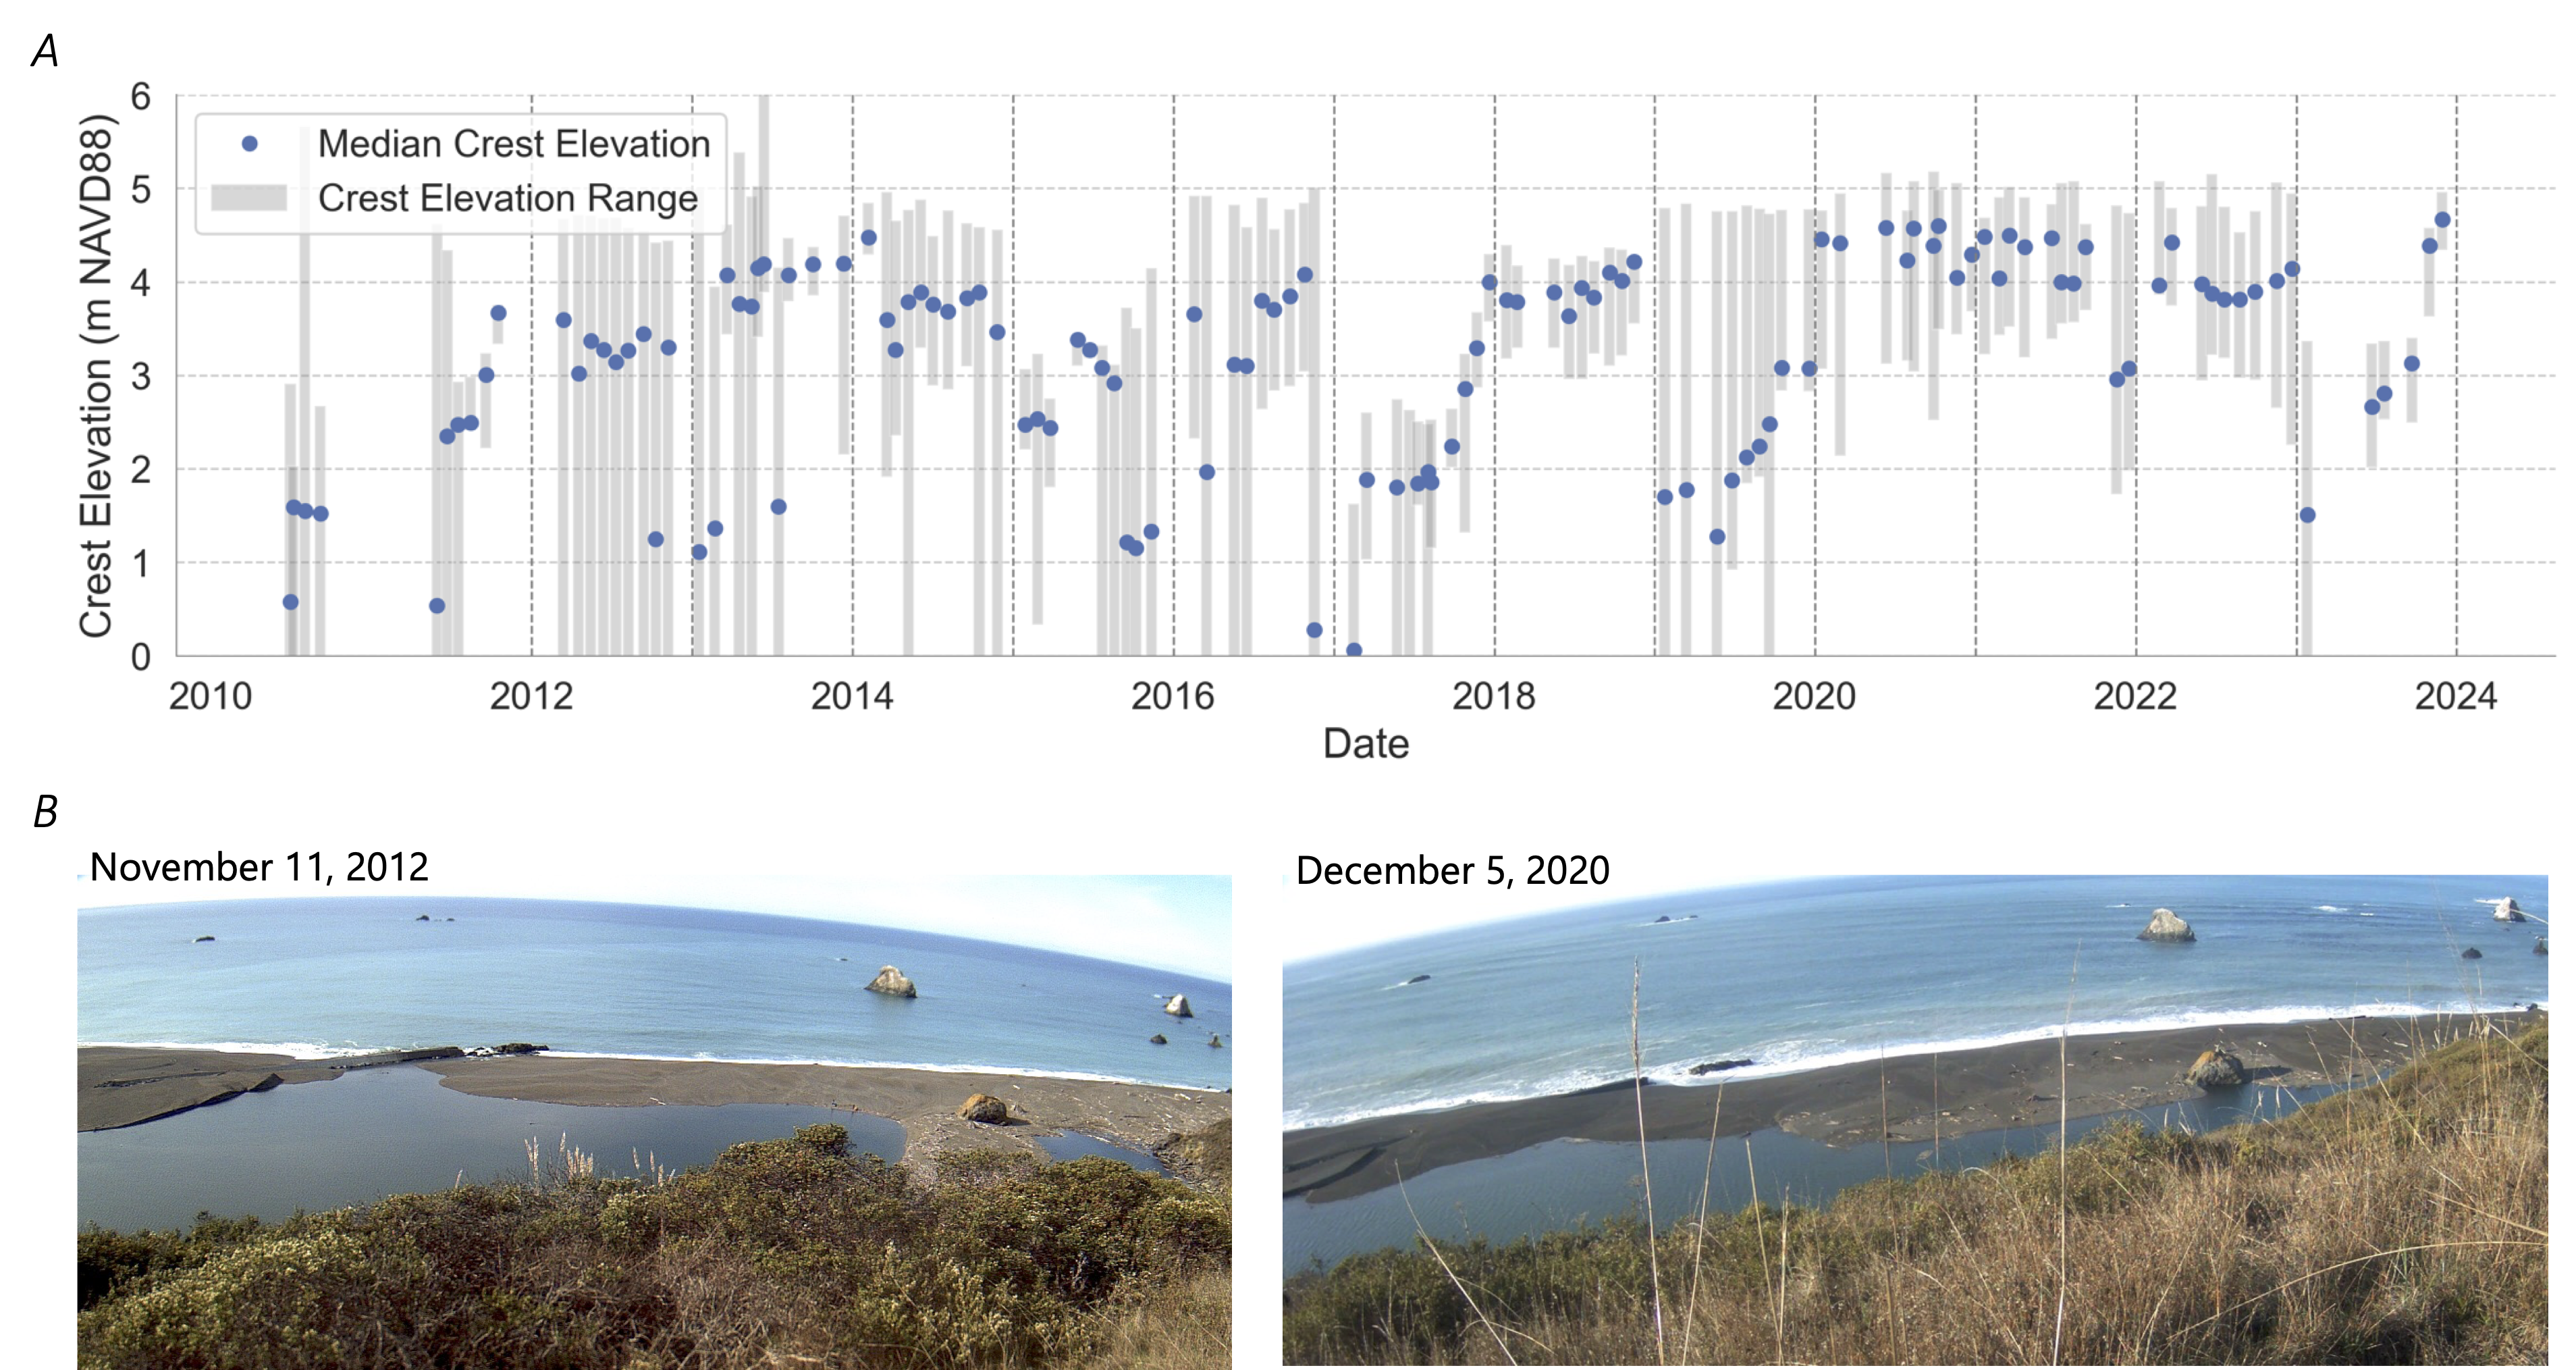
\includegraphics[width = \textwidth]{figures/interannual_variability.png}
    \caption{Berm crest elevation as a function of time, showing the median (blue dots) and range of  four transects across the berm. Photos taken on November 11, 2012 and December 5, 2020, illustrating larger interannual changes in the berm shape.  In 2012, large $\tilde K$ is consistent with a narrowing berm by the jetty.  Likewise, in 2020, small $\tilde K$ is consistent with the wider berm shape.   }
    \label{fig:berm_crest}
\end{figure}


  \begin{figure}
    \centering
    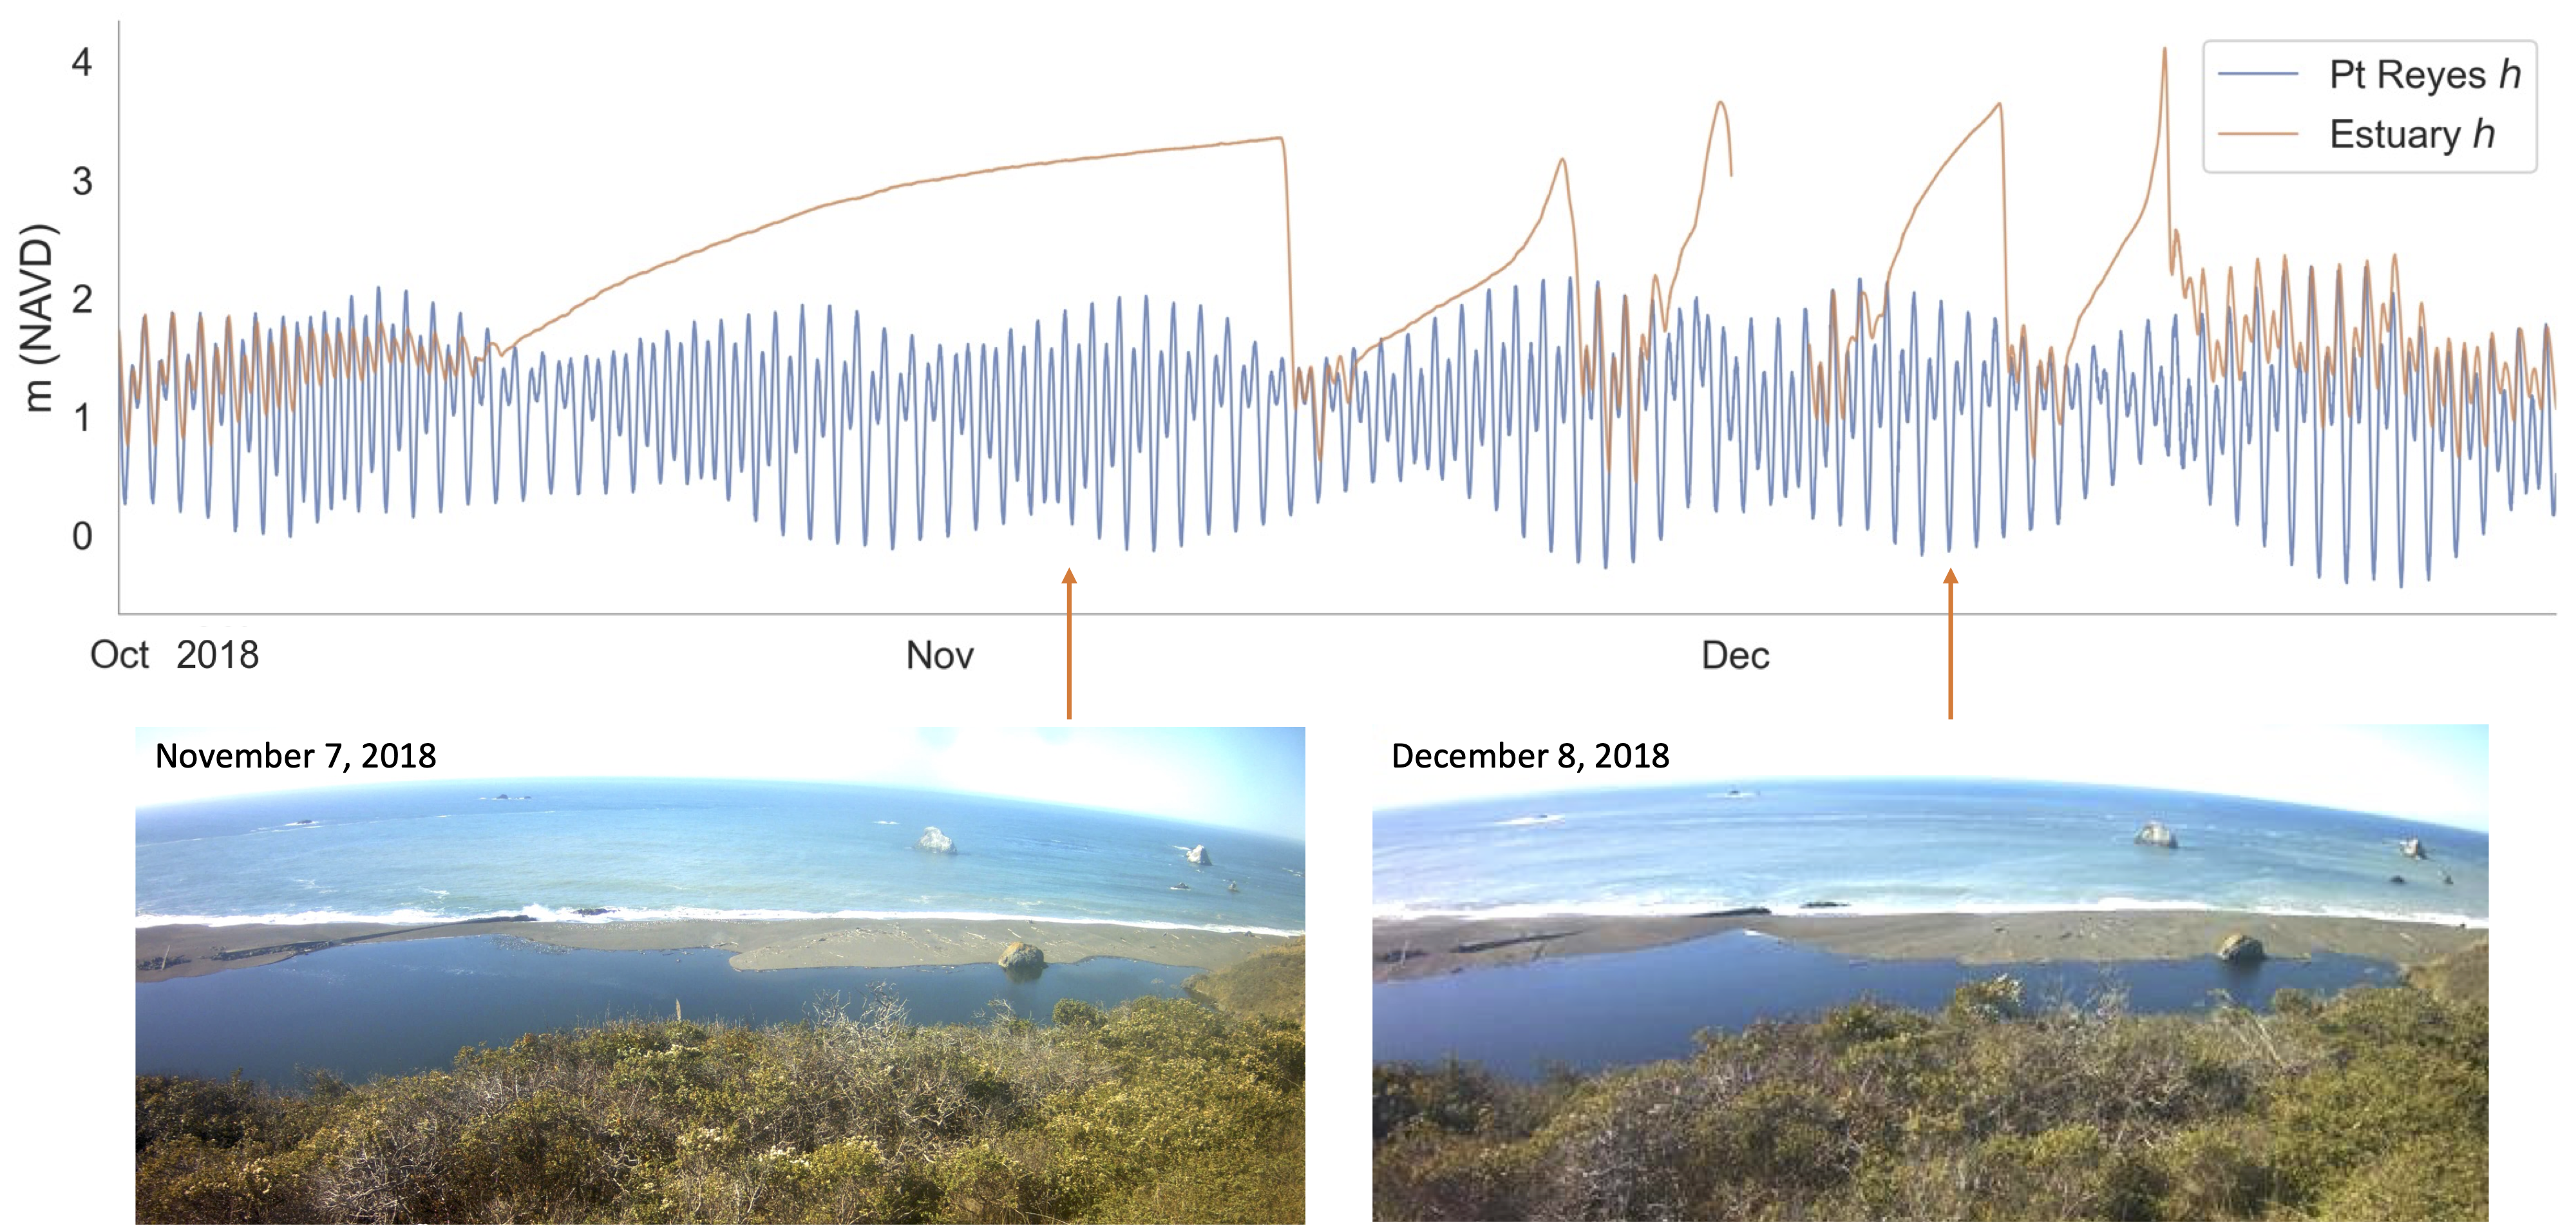
\includegraphics[width = \textwidth]{figures/subsequent_closures.png}
    \caption{Photos taken November 7, 2018 and December 8, 2018, illustrate how the berm shape varies little over subsequent closures within the same year. }
    \label{fig:2018_closures}
\end{figure}


In the absence of wave overwash,  day-to-day variability in $S$ is on the order of 0.1 m$^3$/s, which is an order of magnitude smaller than typical seepage rates. More persistent sources of uncertainty in seepage estimates include: 
(i)  evaporative loss from the estuary, 
(ii) unaccounted for wave overwash events, 
(iii) groundwater exchange, and 
(iv) differences in ocean water level between Point Reyes gauge and the Russian River mouth associated with wind and wave setup. We assessed whether errors in ocean level estimates due to wind or wave setup could  explain outliers in $S$ estimates, and found no clear relationship with short-lived wind or wave events that may account for local water level setup. While unlikely to change the above-described mass balance that exhibits a tight relation between head and through-berm seepage, the role of groundwater fluxes remains an uncertainty in general and it may be an important term in other intermittently closed estuaries.
% Groundwater influx may occur as estuary water levels rise. However, we did not include groundwater fluxes in the mass balance equation (Equation \ref{eq:dVdt}), as the results indicate a well-behaved Darcy-like seepage loss during closures, while groundwater influx is less likely to exhibit a linear relationship with estuary water levels.

With the observed seepage rates and dependence on estuary water level, a steady-state balance could occur in the Russian River estuary (i.e., where river inflow is balanced by seepage through the berm, allowing for persistent closures). The berm is often high enough for estuary water level to rise 2-3 m above ocean water levels. Under these conditions, seepage could be as high as 2 or 3 m$^3$/s (100-140 cfs, using overall best-fit value for $\tilde K$ of 1.06; Figure 5D), which is greater than typical summer river flow rates that are managed to maintain adequate water availability in the lower river.
However, this steady state is rarely achieved, because 
the estuary mouth is breached mechanically before estuary water level reaches 2.74 m NGVD29 (1.9 m NAVD), limiting the maximum seepage rates.
At this level, seepage can account for a loss of approximately 2 m$^3$/s, which is less than typical summer river flows. An exception is in the 2014 drought year, when river flow rate decreased to  approximately 2 m$^3$/s and long closures were observed (Table 1). For the first 10 days of October, seepage balanced river inflow and the water level remained nearly constant in the estuary increasing $\approx$0.2 m from 2.7 to 2.9 m NAVD (see Figure \ref{fig:overwash}). 
%A steady state also persisted in June 2024 when a long, thin secondary berm developed prior to closure. 
%In years with higher river flow, a steady state could potentially  be achieved if water level rose to about 3 m above ocean water level (assuming $Q_r = 3$ m$^3$/s and $\tilde K$ = 1 m$^2$/s, $\Delta h = S / \tilde K = 3 $ m). 

Steady-state conditions likely occurred prior to human modifications, as closures could start in spring and persist for months through the summer low-flow months. Alternatively, closure may have persisted with the estuary water level over-topping the crest of the berm (i.e., perched state), but with high seepage allowing for an overflow rate low enough that the berm was not scoured. For example, in this perched estuary state, if 0.5 m$^3$/s flowed over the sand barrier as a 10 m wide and 0.1 m deep flow with velocities below 0.5 m/s, flow would likely  not scour the sand and the barrier would remain in place. 
 
Prolonged closures allow a freshwater layer (epilimnion) to develop in the estuary, which offers critical habitat for freshwater-acclimated young steelhead \citep{largier20205}. Further, a cool, moderate-salinity metalimnion also can develop, offering habitat for smolts to grow prior to leaving the estuary and entering the ocean in the fall. The deep and cold hypolimnion becomes anoxic beneath very strong stratification that precludes mixing and re-oxygenation, without any significant photosynthetically active radiation. If the present management protocol continues under rising sea level, the maximum head difference between estuary and ocean will be reduced, and the maximum possible seepage will be further constrained.  This may result in shorter closure events, with less persistent and thinner epilimnion and metalimnion layers, reducing valuable habitat for juvenile salmonids.  

% might be worth mentioning in Section 1 that the water balance in lagoons like the Russian could change in the future if evaporative losses increase (due to warmer temps), and if summertime inflows decrease and the annual 'dry' season gets longer (I think this is where the GCM models were heading last I saw, but should confirm). If those are both true, seepage loss rates could contribute to longer-duration closure events, and lower water levels in the lagoon, compared to existing conditions.

 Seepage losses are likely significant in other ICEs where the water level rises significantly above the ocean water level, which occurs where river inflow exceeds evaporative losses during closure periods.  Different barrier configurations, in terms of dimensions and sediment types, are expected to result in different flow rates.  Likewise, other ICEs may exhibit differences in how $\tilde K$ changes over seasons and years, due to clogging and/or changes in berm shape. While some data exist for similar water-balance analyses in other California ICEs, new work should also include data collection that can better define and demonstrate controls on the seepage process.

\label{sec:discussion}

\section{Conclusion}

This study combined a multi-year record of the daily condition of the Russian River inlet, estuary water level, and river discharge data to compute seepage rates during estuary closures.
We then estimated an integrated hydraulic conductivity $\tilde K$ by regression of the seepage rate $S$ on the head difference between ocean and estuary, $\Delta h$. 
Aggregating over 35 closure events with durations of at least six days, we find that the average seepage rate is $S = 1.06 \Delta h$.
We suggest that interannual variability in $\tilde K$ reflects variations in berm shapes, and seasonal variability reflects changes in the composition and hydraulic conductivity of the berm (e.g., clogging by fine particles).

\section{Acknowledgments}
We are grateful for funds and data received from the Sonoma County Water Agency to UC Davis Bodega Marine Laboratory and Environmental Science Associates for monitoring of estuary conditions in the Russian River. UC Davis is also grateful for funds received from the California Department of Parks and Recreation for monitoring and understanding water levels in Californian estuaries. The authors thank Jessica Martini-Lamb, Chris Delaney, Michael Koohafkan, and Elinor Twohy for dialog, insight, and assistance in this study.
 
%% If you have bibdatabase file and want bibtex to generate the
%% bibitems, please use
%%
 \bibliographystyle{elsarticle-harv} 
 \bibliography{local.bib}


\end{document}

\endinput
%%



 
 % We  compare the  $\tilde K$  values estimated using mass balance approaches to  back-of-the-envelope estimates using Darcy's law, assuming $K = 410$ m/day for a mix of gravel and sand \citep{masters1991introduction}, $L_b = 300 $ m for the length of the berm \citep{behrens2009characterization}, $W_b = 50$ m for the berm width, and $h_b = 10$ m for the a hydraulically-active depth,  combining yields $\tilde K = K W_b h_b/L_b = 0.28$ m$^3$/s.  This estimate is smaller than typical $\tilde K$ values determined by  mass balance, which may in part be attributable to pipes and other preferential flow paths.  

% The study ignores groundwater surface water interactions. While the linear relationship between $\Delta h$ and $S$ suggests that seepage is a dominant factor, this remains a  study limitation. Further mapping of aquifers and their connections to the river/estuary system, along with models that resolve groundwater-surface water interactions, could better distinguish seepage from groundwater fluxes.

% The study finding that seepage rates tend to increase during closures has  management implications.  The ability to estimate steady state seepage can inform decision-making about if/when to breach the berm.
% An important question is therefore, what is the steady state seepage rate for a given berm shape? 
